% documentclass options:
% ngerman is needed for hyphenation if the thesis contains parts written in German
% BCOR is binding correction
% if you'd rather have a one sided thesis, add `oneside' to the documentclass
\documentclass[11pt,
  a4paper,
  % parskip=half, % This is some extra vertical space between paragraphs, the suggestion is 2cm which is really ugly, so we use what koma script gives us
  % you can also set it to full for even more space. But there is a bad tex style decision: parskip also changes the spacing between listitems such as
  % enumerate and itemize. For this purpose we include the enumitem package and set itemsep=.5em, of course you can change this
  BCOR=10mm,
  english]{book}
\usepackage[english]{babel} % If you write mainly in english change order to ngerman, english
% Include of titling must happen before \title etc.
% that's why it's not in setup.tex
\usepackage{titling}
\title{Distributed assertion checking in smart contracts}
\author{Tamara Bernhardt}

% include all packages and define commands in setup.tex

%------------------------------------------------------------------------------
%       package includes
%------------------------------------------------------------------------------
    % font encoding is set up for pdflatex, for other environments see
    % http://tex.stackexchange.com/questions/44694/fontenc-vs-inputenc
    \usepackage[T1]{fontenc}  % 8-bit fonts, improves handling of hyphenations
    \usepackage{lmodern}
    \usepackage[utf8x]{inputenc}
    % provides `old' commands for table of contents. Eases the ability to switch
    % between book and scrbook
    % cross-referencing
    \usepackage{xr}


    % ------------------- layout, default -------------------
    % adjust the style of float's captions, separated from text to improve readabilty
    \usepackage[labelfont=bf, labelsep=colon, format=hang, textfont=singlespacing]{caption}
    % With format = hang your caption will look like this:
    % Figure 1: Lorem ipsum dolor sit amet,
    %           consectetuer adipiscing elit.
    %           Ut purus elit, vestibulum
    % If you instead want
    % Figure 1: Lorem ipsum dolor sit amet,
    % consectetuer adipiscing elit. Ut purus
    % elit, vestibulum
    % change to format=plain
    \usepackage{chngcntr}  % continuous numbering of figures/tables over chapters
    \counterwithout{equation}{chapter}
    \counterwithout{figure}{chapter}
    \counterwithout{table}{chapter}

    % Uncomment the following line if you switch from scrbook to book
    % and comment the setkomafont line
    \usepackage{titlesec}  % remove "Chapter" from the chapter title
    \titleformat{\chapter}[hang]{\bfseries\huge}{\thechapter}{2pc}{\huge}
    % \setkomafont{chapter}{\normalfont\bfseries\huge}

    \usepackage{setspace}  % Line spacing
    \onehalfspacing
    % \doublespacing  % uncomment for double spacing, e.g. for annotations in correction

    % ------------------- functional, default-------------------
    \usepackage{natbib}
    \usepackage[dvipsnames]{xcolor}  % more colors
    \usepackage{array}  % custom format per column in table - needed on the title page
    \usepackage{graphicx}  % include graphics
    \usepackage{subfig}  % divide figure, e.g. 1(a), 1(b)...
    \usepackage{amsmath}  % |
    \usepackage{amsthm}   % | math, bmatrix etc
    \usepackage{amsfonts} % |
    \usepackage{calc}  % calculate within LaTeX
    \usepackage[unicode=true,bookmarks=true,bookmarksnumbered=true,
                bookmarksopen=true,bookmarksopenlevel=1,breaklinks=false,
                pdfborder={0 0 0},backref=false,colorlinks=false]{hyperref}
	\usepackage{listings}
	\usepackage{tabularx}
	\usepackage{makecell}
	\usepackage{upquote}

    %==========================================
    % You might not need the following packages, I only included them as they
    % are needed for the example floats
    % ------------------- functional, custom -------------------
    \usepackage{algorithm,algpseudocode}
    \usepackage{bm}  % bold greek variables (boldmath)
    \usepackage{tikz}
    \usetikzlibrary{positioning}  % use: above left of, etc

    % Improves general appearance of the text
    \usepackage[protrusion=true,expansion=true, kerning]{microtype}
    \usepackage{enumitem}

	\usepackage{csquotes}
	\usepackage{scrhack}

%------------------------------------------------------------------------------
%       (re)new commands / settings
%------------------------------------------------------------------------------
    % ----------------- referencing ----------------
    \newcommand{\secref}[1]{Section~\ref{#1}}
    \newcommand{\chapref}[1]{Chapter~\ref{#1}}
    \renewcommand{\eqref}[1]{Equation~(\ref{#1})}
    \newcommand{\figref}[1]{Figure~\ref{#1}}
    \newcommand{\tabref}[1]{Table~\ref{#1}}
    \newcommand{\lstref}[1]{Listing~\ref{#1}}
    %\newcommand{\algref}[1]{Algorithm~\ref{#1}}
    \newcommand*{\captionsource}[2]{%
  		\caption[{#1}]{%
    	#1%
    	\\\hspace{\linewidth}%
    	Source: #2%
  		}%
	}

    % ------------------- colors -------------------
    \definecolor{darkgreen}{rgb}{0.0, 0.5, 0.0}
    % Colors of the Albert Ludwigs University as in
    % https://www.zuv.uni-freiburg.de/service/cd/cd-manual/farbwelt
    \definecolor{UniBlue}{RGB}{0, 74, 153}
    \definecolor{UniRed}{RGB}{193, 0, 42}
    \definecolor{UniGrey}{RGB}{154, 155, 156}
    \definecolor{cverbbg}{gray}{0.93}

    % ------------------- layout -------------------
    % prevents floating objects from being placed ahead of their section
    \let\mySection\section\renewcommand{\section}{\suppressfloats[t]\mySection}
    \let\mySubSection\subsection\renewcommand{\subsection}{\suppressfloats[t]\mySubSection}


    % ------------------- marker commands -------------------
    % ToDo command
    \newcommand{\todo}[1]{\textbf{\textcolor{red}{(TODO: #1)}}}
    \newcommand{\extend}[1]{\textbf{\textcolor{darkgreen}{(EXTEND: #1)}}}
    % Lighter color to note down quick drafts
    \newcommand{\draft}[1]{\textbf{\textcolor{NavyBlue}{(DRAFT: #1)}}}
    \newcommand{\move}[1]{\textbf{\textcolor{Orange}{(MOVE?: #1)}}}


    % ------------------- math formatting commands -------------------
    % define vectors to be bold instead of using an arrow
    \renewcommand{\vec}[1]{\mathbf{#1}}
    \newcommand{\mat}[1]{\mathbf{#1}}
    % tag equation with name
    \newcommand{\eqname}[1]{\tag*{#1}}


    % ------------------- pdf settings -------------------
    % ADAPT THIS
    \hypersetup{pdftitle={\thetitle},
                pdfauthor={\theauthor},
                pdfsubject={Master's thesis at the Albert Ludwig University of Freiburg},
                pdfkeywords={blockchain, smart contract},
                pdfpagelayout=OneColumn, pdfnewwindow=true, pdfstartview=XYZ, plainpages=false}


    %==========================================
    % You might not need the following commands, I only included them as they
    % are needed for the example floats

    % ------------------- Tikz styles -------------------
    \tikzset{>=latex}  % arrow style


    % ------------------- algorithm ---------------------
    % Command to align comments in algorithm
    \newcommand{\alignedComment}[1]{\Comment{\parbox[t]{.35\linewidth}{#1}}}
    % define a foreach command in algorithms
    \algnewcommand\algorithmicforeach{\textbf{foreach}}
    \algdef{S}[FOR]{ForEach}[1]{\algorithmicforeach\ #1\ \algorithmicdo}

    % line spacing should be 1.5
    \renewcommand{\baselinestretch}{1.5}

    % set distance between items in a list, for more details see the
    % enumitem package: https://www.ctan.org/pkg/enumitem
    \setlist{itemsep=.5em}

% Copyright 2017 Sergei Tikhomirov, MIT License
% https://github.com/s-tikhomirov/solidity-latex-highlighting/

\usepackage{listings, xcolor}

\definecolor{verylightgray}{rgb}{.97,.97,.97}

\lstdefinelanguage{Solidity}{
	keywords=[1]{anonymous, assembly, assert, balance, break, call, callcode, case, catch, class, constant, continue, constructor, contract, debugger, default, delegatecall, delete, do, else, emit, event, experimental, export, external, false, finally, for, function, gas, if, implements, import, in, indexed, instanceof, interface, internal, is, length, library, log0, log1, log2, log3, log4, memory, modifier, new, payable, pragma, private, protected, public, pure, push, require, return, returns, revert, selfdestruct, send, solidity, storage, struct, suicide, super, switch, then, this, throw, transfer, true, try, typeof, using, value, view, while, with, addmod, ecrecover, keccak256, mulmod, ripemd160, sha256, sha3}, % generic keywords including crypto operations
	keywordstyle=[1]\color{blue}\bfseries,
	keywords=[2]{address, bool, byte, bytes, bytes1, bytes2, bytes3, bytes4, bytes5, bytes6, bytes7, bytes8, bytes9, bytes10, bytes11, bytes12, bytes13, bytes14, bytes15, bytes16, bytes17, bytes18, bytes19, bytes20, bytes21, bytes22, bytes23, bytes24, bytes25, bytes26, bytes27, bytes28, bytes29, bytes30, bytes31, bytes32, enum, int, int8, int16, int24, int32, int40, int48, int56, int64, int72, int80, int88, int96, int104, int112, int120, int128, int136, int144, int152, int160, int168, int176, int184, int192, int200, int208, int216, int224, int232, int240, int248, int256, mapping, string, uint, uint8, uint16, uint24, uint32, uint40, uint48, uint56, uint64, uint72, uint80, uint88, uint96, uint104, uint112, uint120, uint128, uint136, uint144, uint152, uint160, uint168, uint176, uint184, uint192, uint200, uint208, uint216, uint224, uint232, uint240, uint248, uint256, var, void, ether, finney, szabo, wei, days, hours, minutes, seconds, weeks, years},	% types; money and time units
	keywordstyle=[2]\color{teal}\bfseries,
	keywords=[3]{block, blockhash, coinbase, difficulty, gaslimit, number, timestamp, msg, data, gas, sender, sig, value, now, tx, gasprice, origin},	% environment variables
	keywordstyle=[3]\color{violet}\bfseries,
	identifierstyle=\color{black},
	sensitive=false,
	comment=[l]{//},
	morecomment=[s]{/*}{*/},
	commentstyle=\color{gray}\ttfamily,
	stringstyle=\color{red}\ttfamily,
	morestring=[b]',
	morestring=[b]"
}

\lstdefinestyle{Solidity}{
	backgroundcolor=\color{verylightgray},
	extendedchars=true,
	basicstyle=\footnotesize\ttfamily,
	showstringspaces=false,
	showspaces=false,
	numbers=left,
	numberstyle=\footnotesize,
	numbersep=9pt,
	tabsize=2,
	breaklines=true,
	showtabs=false,
	captionpos=b
}

\usepackage{listings, xcolor}

\definecolor{verylightgray}{rgb}{.97,.97,.97}

\lstdefinelanguage{Michelson}{
	keywords=[1]{parameter, storage, code},
	keywordstyle=[1]\color{blue}\bfseries,
	keywords=[2]{address, unit, never, bool, int, nat, string, chain_id, bytes, mutez, key_hash, key, signature, timestamp,
	option, or, pair, list, set, operation, ticket, lambda, map, big_map, sapling_transaction, sapling_state, bls12_381_g1,
	bls12_381_g2, bls12_381_fr},	% types; money and time units
	keywordstyle=[2]\color{teal}\bfseries,
	keywords=[3]{Do, call, assert},
	keywordstyle=[3]\color{violet}\bfseries,
	identifierstyle=\color{black},
	sensitive=false,
	comment=[l]{//},
	morecomment=[s]{(*}{*)},
	commentstyle=\color{gray}\ttfamily,
	stringstyle=\color{red}\ttfamily,
	morestring=[b]',
	morestring=[b]"
}

\lstset{
	language=Michelson,
	backgroundcolor=\color{verylightgray},
	extendedchars=true,
	basicstyle=\footnotesize\ttfamily,
	showstringspaces=false,
	showspaces=false,
	numbers=left,
	numberstyle=\footnotesize,
	numbersep=9pt,
	tabsize=2,
	breaklines=true,
	showtabs=false,
	captionpos=b
}

\usepackage{listings, xcolor}

\definecolor{verylightgray}{rgb}{.97,.97,.97}

\lstdefinelanguage{Assertion}{
	keywords=[1]{entrypoint, assert, if, else, true, false, forall, exists},
	keywordstyle=[1]\color{blue}\bfseries,
	keywords=[2]{address, unit, never, bool, int, nat, string, chain_id, bytes, mutez, key_hash, key, signature, timestamp,
	option, or, pair, list, set, operation, lambda, map, big_map},	% types; money and time units
	keywordstyle=[2]\color{teal}\bfseries,
	keywords=[3]{left, right, some, none, cons, nil, _},
	keywordstyle=[3]\color{violet}\bfseries,
	identifierstyle=\color{black},
	sensitive=false,
	comment=[l]{//},
	morecomment=[s]{(*}{*)},
	commentstyle=\color{gray}\ttfamily,
	stringstyle=\color{red}\ttfamily,
	morestring=[b]',
	morestring=[b]"
}


\begin{document}
    \pagestyle{empty} % no header and no page number
    % disable hyper links to remove warning "destination with same identifier"
    % this means within this section nothing can be referenced with a hyperlink
    \hypersetup{pageanchor=false}

    % enable/disable, depending on your chosen language
    
\begin{titlepage}
\begin{center}

\newcommand{\HorizontalLine}{\rule{\linewidth}{0.3mm}}

{\Large Master's Thesis}\\[1.3cm]


% _____________________________________________________________________________
\HorizontalLine \\[0.4cm]
% Write your title in a fancy way like this if you want to customize it, otherwise simply let tex do it for you
% \begin{spacing}{3}
%     {\huge \bfseries The Long, Long } \\
%     {\huge \bfseries Long Long} \\
%     {\huge \bfseries Title}\\
% \end{spacing}
{ \huge \bfseries \thetitle }
\HorizontalLine \\[1.5cm]
% _____________________________________________________________________________


{\Huge \theauthor} \\[2cm]


\begin{tabular}[hc]{>{\huge}l >{\huge}l}
  Examiner: & Prof. Dr. Peter Thiemann \\[0.3cm]
  2nd Examiner: & Prof. Dr. Andreas Podelski \\[0.3cm]
  Advisers: & \todo{lla} \\[1.2cm]
\end{tabular}
\vfill  % move the following text to the bottom

\Large {
    Albert-Ludwigs-University Freiburg\\
    Faculty of Engineering\\
    Department of Computer Science\\
    Chair for Programming Languages\\[1cm]
}
\end{center}
\end{titlepage}

\thispagestyle{empty}
% title page back
\ \vfill \ \\  % at least one space required before vfill
\
\textbf{Writing period}            \smallskip{} \\
01.\,10.\,2020 -- 31.\,03.\,2021 \todo   \bigskip{} \\
\
\textbf{Examiner}                  \smallskip{} \\
Prof. Dr. Peter Thiemann               \bigskip{} \\
\
\textbf{2nd Examiner}                  \smallskip{} \\
Prof. Dr. Andreas Podelski


    \pagestyle{plain} % remove chapter name from top, page number at the bottom
    % use \pagestyle{headings} for having the chapter on top of the pages
    % if you wang a more fancy header use \usepackage[automark,headsepline]{scrlayer-scrpage}
    % and read about it in the KOMA script documentation, https://www.ctan.org/pkg/koma-script
    \frontmatter  % roman page numbers
    % official declaration from the examination office; to be sure double
% check the wording on their website
% (https://www.tf.uni-freiburg.de/studies/exams/thesis/thesis_formatting.html#erklaerung)

\chapter*{Declaration}

I hereby declare that I am the sole author and composer of my thesis and that no other sources or learning aids, other than those listed, have been used. Furthermore, I declare that I have acknowledged the work of others by providing detailed references of said work.  \newline
I hereby also declare that my Thesis has not been prepared for another examination
or assignment, either wholly or excerpts thereof.
\\[3\normalbaselineskip]
\begin{tabular}{p{\textwidth/2} l}
  \rule{\textwidth/3}{0.4pt}   &   \rule{\textwidth/3}{0.4pt} \\
  Place, Date                  &   Signature
\end{tabular}

    \chapter*{Abstract}
Modern blockchains provide a platform for building sophisticated applications with smart contracts. Because transactions are processed at every node in the network, the quantity and complexity of computations, which can be performed by smart contracts, are limited. Furthermore, complex contracts can generate high transaction costs for the user. To overcome this limitation and improve cost efficiency, blockchain-based applications could move computations to an off-chain component and only process the result on the blockchain. This thesis proposes a processing model for the Tezos blockchain, which engages the validators of the network in a distributed effort to verify a submitted off-chain computation. Based on a specification of properties, the validators are challenged to find a counterexample by asserting these properties for independent subsets of the result. This reduces the computational effort on the blockchain to the verification of the result, rather than the computation of the result itself. Moreover, by implementing a distributed scheme, each node only processes a fraction of the verification. For this processing model, this thesis contributes a domain-specific language to express explicit assertions for off-chain computations and specifies a processing pipeline to transform and compile these assertions into smart contracts. These contracts conduct a point-wise search for a counterexample and are called during the verification mechanism. The provided proof-of-concept implementation of this pipeline targets Tezos, but is by design extendible for other blockchains supporting smart contracts.
    \tableofcontents
    \listoffigures
    % \listoftables
    % \listofalgorithms
    \hypersetup{pageanchor=true}  % re-enable hyperlinking

    \mainmatter  % Arabic page numbers
    \chapter{Introduction}\label{chap:introduction}
Headed by Bitcoin in 2009 \cite{bitcoin-whitepaper}, the first generation of blockchain technology emerged in form of cryptocurrencies. However, their transactions are mostly limited to simple monetary transactions or registration of assets or ownerships \cite{alharby_blockchain_2017}. More recent blockchains, considered as the second generation, aim to provide a platform for building more sophisticated and complex applications on top of the technology. Some prominent examples for such blockchains are Ethereum \cite{eth-whitepaper}, Tezos \cite{goodman_tezos_2014} or Cardano \cite{cardano_essay}, which plans to introduce smart contracts in an update this year \cite{cardano_alonzo}. Blockchain-based applications are built with smart contracts, programs written in Turing-complete languages. Running a smart contract, though, generates costs proportional to the amount and complexity of computations, as well as its storage usage \cite{alharby_blockchain_2017}. These fees, often measured in a unit called ``gas'', have to be paid for by the user in order to compensate the miners for their efforts \cite{narayanan_bitcoin}. This creates a powerful incentive to keep smart contracts simple and efficient, while in reality, meaningful applications still might need to perform some resource intensive computations. Not only can such applications generate unsustainable costs when executed on the blockchain, but may also reach gas limits imposed by the blockchain's protocol. \\
In order to avoid these costs and restrictions, such an application could perform some computations outside of the blockchain context (i.e., off-chain) and only submit the results to a smart contract as an input parameter for further processing or recording. By trusting that the submitted results are correct, this approach raises both safety and security issues. Invalid results can be submitted unintentionally as a result of a wrong computation, or a third party may pass them intentionally to cause harm or take advantage. Consequently, submitted parameters should be checked for assumed properties before the smart contract is executed. Although in many cases, verifying a solution takes less time than computing the result itself (cf. NP-hard problems \cite{nph_problems} or sorting algorithms \cite{review_sorting}\cite{cpp_issorted}), the generated costs for checking the validity increase with the size of the input. \\
Consider the smart contract \texttt{Example}, which is shown in \lstref{lst:prime} and features a function \texttt{f}. The function takes an input value \texttt{p} of type integer and should make use of the assumption that \texttt{p} is a prime number.
\begin{lstlisting}[caption=Smart contract with a function that expects a prime number \cite{thiemann_2020}, numbers=none, language=Solidity, label=lst:prime]
contract Example {
	function f ( int p ) public {
	// assume p is prime
	...
	}
}
\end{lstlisting}
This assumption ``$p$ is a prime number'' can be expressed with the following explicit assertion in predicate logic: 
\begin{equation}\label{eq:prime}
    (\forall n) (2 \le n \le \sqrt{p}) \Rightarrow (p \% n) \neq 0
\end{equation}
To check whether this property holds for $p$, the contract has to execute a loop over the range $[2, \sqrt{p}]$. Assuming that computing the body of the loop takes constant time, this test has a time complexity of $\mathcal{O}(\sqrt{p})$ and therefore generates costs linear in $\sqrt{p}$ on top of the cost for executing the actual contract. Thus, a mechanism is required that allows the smart contract to make use of the result computed by an off-chain source, without having to check its validity locally with scaling costs.

\section{A distributed approach for assertion checking}
A more efficient way to solve the issue at hand could be to engage the validators of the blockchain into a distributed effort to find a counterexample. If no counterexample could be found by any validator, the assumption is considered to be valid and the execution of the contract may resume. On the other hand, an identified counterexample is made public on the peer-to-peer network and thus cancels the contract execution (i.e., the transaction fails). \\
In order to find a counterexample, the formula in \eqref{eq:prime} has to be transformed to its negation:
\begin{equation}\label{eq:prime_neg}
	(\exists n) (2 \le n \le \sqrt{p}) \wedge (p \% n) = 0
\end{equation}

Each validator then checks the inverse property $(p \% n) = 0$ point-wise for some random $n$ within the given boundaries $2 \le n \le \sqrt{p}$. If a validator finds a counterexample, i.e., a value for $n$ where the reminder is $0$, it posts an objection to the network. For each involved validator, the constant cost of generating one random number and calculating one division have to be paid, which is independent from $p$. \\
However, distributed assertion checking is not only applicable for parameters or properties of dynamic size. Function \texttt{find} of contract \texttt{Sorted}, shown in \lstref{lst:sorted}, expects a statically sized array of integers and a single integer value. In order to find the value \texttt{v} in \texttt{a} more efficiently, the array is assumed to be sorted. 

\begin{lstlisting}[caption=Smart contract expecting a sorted array \cite{thiemann_2020}, numbers=none, language=Solidity, label=lst:sorted]
contract Sorted {
  function find ( int [50] a , int v ) public {
    // assume a is sorted
    ...
  }
}
\end{lstlisting}

The explicit assertion of this assumption (in the variant of an ascending sorting) can be expressed as follows in predicate logic:
\begin{equation}\label{eq:sorted}
	(\forall n) (0 \leq n < |a| - 1) \Rightarrow a[n] \leq a[n+1]
\end{equation}

Even though the assertion can be checked in a loop in $\mathcal{O}(1)$, the constant factor is not negligible. Hence, the same approach can be applied here by considering the negation and have the validators search for counterexamples, checking random values for $n$:
 
\begin{equation}\label{eq:sorted_neg}
	(\exists n) (0 \leq n < |a| - 1) \wedge a[n] > a[n+1]
\end{equation}

Since the validators sample the domain randomly, the absence of a counterexample doesn't prove that the assumption is correct; the validation is only probabilistic and the reliability depends on the number of validators in the network. This corresponds to the principle of Bloom filters, where a queried element is either ``certainly not'' or ``possibly'' a member of a defined set \cite{blustein_bloom_2002}. In the case of assertion checking, we consider the assumption to be either definitely not or possibly valid. The probability of false positives in Bloom filters is an approximate function of the filter size and the number of inserted elements, supposing an optimal number of hash functions have been implemented. Tuning these parameters is a trade-off between making the filter more reliable, i.e., lowering its error rate, and space efficiency \cite{blustein_bloom_2002}. The same applies, with some reservations, to distributed assertion checking: less samples keep the gas consumption to a minimum, whereas more samples increase the probability that an existing counterexample is found. Referring to the example of sorted lists,  the probability of false positives depends on the size of the list $a$ and the number of validators $m$.

The importance of the former parameter becomes apparent when considering the worst case scenario of the same example. Assuming the array is unsorted at exactly one position - the probability that the each of the $m$ validators independently check this position is $\frac{1}{|a|}$, whereas the probability of all of them checking any other position $\frac{|a|-1}{|a|}$. If the random generator chooses each value for $n$ independently from a uniform distribution, the probability that the counterexample is not detected by any validator converges to 0 if the number of validators approaches infinity \cite{thiemann_2020}:
\begin{equation}\label{eq:limes_validators}
	\lim_{m\to\infty} \left(\frac{|a|-1}{|a|}\right)^m = 0
\end{equation}

\section{Objective}
This thesis proposes a model for the portrayed approach of a distributed assertion checking scheme, to make more efficient use of off-chain computations. In this model, results of such computations are validated on-chain by the validators of the network. In order to do so, they invoke assertion smart contracts which point-wise check whether the result satisfies certain properties. When claiming an assertion failure, a validator publishes a counterexample to be scrutinized by the other validators. If they come to a consensus about the invalidity, the result is rejected. Provided that the assertion is cheaper than the computation itself, the purpose of this proposal is not only to reduce financial costs for the users, but also to overcome limitations in scalability. 

The realisation of such assertions consists of an off-chain and an on-chain component. The off-chain component is a toolchain to specify, integrate and generate assertion contracts that can be deployed to the blockchain. It defines of a domain-specific language which allows developers to specify assertions for each entrypoint of a Smart Contract. The toolchain implements a pipeline which transforms the assertion, links it with the Smart Contract and translates it to the Smart Contract language. \\
The on-chain component consists of an amendment of the blockchain protocol to include transactions that can trigger the distributed execution of assertions and implement a consensus mechanism for counterexamples. 

The focus of this thesis is put primarily on the off-chain component, but it elaborates on the protocol design where necessary.  Even though efforts were made to keep the design as generic and re-usable as possible, the implementation targets the Tezos blockchain and its built-in contract language Michelson. On the basis of the design and implementation for Tezos, the thesis evaluates the efficiency and incurred costs of this approach and discusses whether, and under which conditions, they can be competitive versus a centralized assertion approach.

\section{Related work}


\section{Structure overview}
The structure of this thesis is as follows: in the first instance, \chapref{chap:use_cases} defines a set of logical formulas suitable for distributed assertion checking. Given this set, it demonstrates various practical use-cases for such properties and formalizes the costs of checking them locally, s.t. they can later be referenced to assess the efficiency of the distributed approach. \chapref{chap:offline} describes the generic aspects of the off-chain design and infrastructure, i.a. the definition of a syntax to express assertions on top of the logical formulas and how they are transformed to code that checks for counterexamples. Additionally, it analyses the effectiveness of the statistical validation for a given input and provides a formula to compute the lower bound of validators necessary to obtain a reliable result. Subsequently, \chapref{chap:offline_tezos} gives a brief introduction to Tezos, before it covers target specific aspects of the off-chain design. Besides identifying necessary extensions to Michelson's instruction set and virtual machine, it explores various orchestration strategies between assertion and contract code. The chapter closes with a cost analysis of distributed assertion checking on Tezos with the chosen orchestration strategy. In conclusion, the last chapter recaps the achieved results, 
addresses open questions or issues and provides an outlook on upcoming work on this topic.
    \chapter{Use-case analysis}\label{chap:use_cases}
The introduction argued, that validating properties on input parameters can become costly when data structures (such as arrays), certain data types (such as byte sequences) or a range of values have to be iterated. It showed examples for such properties and identified logical formulas containing universal quantification as amenable for distributed assertion checking. Through its domain of discourse, the quantification spans an iteration space whose elements can be checked independently by the validators. As a matter of fact, the same is also valid for existential quantification, even though its negation has a different notion than that of its universal counterpart. The difference between the two is addressed later in this chapter.

The following section formally defines a set of applicable logical formulas for the basic implementation of the distributed assertion checking scheme. Given this set, section \secref{sec:examples} gives some more in-depth examples of such formulas. As a benchmark for the distributed scheme, the last section formalizes the cost incurred by checking formulas on Tezos locally.

\section{Definition of a set of logical formulas}\label{sec:formulae}
The set of formulas, which can be expressed in well-formed assertions, is given in \figref{fig:formulas}. This corresponds, with some restrictions, to the language of second-order predicate logic. Besides universal and existential quantifiers (with exactly one bound variable), the definition contains logical connectives, relational symbols, constant values of a numerical, string or boolean type, variables and the functional symbols for basic arithmetic operations. This set of symbols is rather generic and should be valid for any target blockchain. Specific to the target blockchain are the sets of types $t$ and functional symbols $f$. These can only contain types and operations, which can be translated to instructions of the respective Smart Contract language and interpreted by the blockchain's virtual machine (VM). As an example, the primitive types in Michelson are \texttt{string}, \texttt{nat}, \texttt{int}, \texttt{bytes}, whereas Ethereum's Smart Contract language Solidity  \cite{solidity_docs} additionally supports an \texttt{enum} type and fixed-point numbers.
\begin{align*}
    t &::= \text{primitive data types (existing in the blockchain VM)} \\
    \sigma &::= \forall \mid \exists \\
    \Theta &::= \Phi \mid \sigma (x:t) \Theta \\
    \Phi,\Psi &::= \neg\Phi \mid \Phi \Rightarrow \Psi \mid \Phi\wedge\Psi \mid
    				\Phi\vee\Psi \mid \Phi \oplus \Psi \mid M \rho N \\
    \rho &::= < \mid > \mid \le \mid \ge \mid = \mid \ne \\
    M, N &::= x \mid c \mid M \odot N  \mid f (\overline M) \\
    \odot &::= +\mid -\mid * \mid / \mid \% \\
    c &::= \text{numerical value} \mid string \mid \top \mid \bot \\
    f &::= \text{operations (existing in the blockchain VM)}
\end{align*}
\begingroup\vspace*{-\baselineskip}
\captionof{figure}{Set of logical formulas amenable to distributed assertion checking (based on \cite{thiemann_2020})}
\label{fig:formulas}
\vspace*{\baselineskip}\endgroup

\section{Examples and special cases}\label{sec:examples}
This section contains a subset of use-cases that were collected in collaboration with Julian Veigl for an intermediate report \cite{bernhardt_veigel_2020}. The selection of examples covers different types and compositions of quantifiers, demonstrates different meanings of their negations, identifies special cases and discusses their implications for the implementation of distributed assertion checking.

\subsection{Two numbers are coprime}\label{sec:coprime}
The greatest common divisor ($gcd$) of two non-zero integers $a$ and $b$ is the largest integer that divides both evenly \cite{hardy2008introduction}. A more specific $gcd$-problem is finding two numbers which are coprime, meaning their greatest common divisor is one, i.e., $gcd(a, b) = 1$. In order to verify that two numbers are coprime, it has to be verified that there is no $gcd > 1$, hence the property of coprimeness can be expressed with the following formula in predicate logic:
\begin{equation}\label{eq:coprime-universial}
    (\forall n : int) (2 \le n \le \min(a,b)) \Rightarrow \neg((a \mathbin{\%} n) = 0 \land (b \mathbin{\%} n) = 0)
\end{equation}
Assuming it takes constant time to calculate the two remainders, checking whether two numbers satisfy this property takes linear time, i.e. $\mathcal{O}(n)$, and depends on the size of the smaller number.

When checking the assumption through a distributed effort instead, the validators consider its negation:
\begin{equation}\label{eq:coprime-existential}
    (\exists n : int) (2 \le n \le \min(a,b)) \land (a \mathbin{\%} n) = 0 \land (b \mathbin{\%} n) = 0
\end{equation}
If, within the given domain, this condition is true for a random value for $n$, the respective validator has found a counterexample.

\subsection{Heap property}
Heaps \cite{dict_heap} are data structures based on trees and can appear in two varieties: min and max heaps. Both can be represented as binary trees and have to satisfy the heap property: in a max heap, any given node holds a value lower or equal than that of its parent, whereas in a min heap, it is greater or equal \cite{dict_heap_property}. Binary heaps are often implemented as an array, with the root of the tree stored at index 0. The relatives of a node \texttt{k} can be accessed as follows:
\begin{lstlisting}[language=Solidity, numbers=none, caption=Access a binary heap in array representation]
heap_array[(k-1)/2] // Get parent of node k
heap_array[(k*2)+1] // Get left child of node k
heap_array[(k*2)+2] // Get right child of node k
\end{lstlisting}
The min heap property for a binary heap stored in an array $a$, for instance, can be expressed in predicate logic with the following formula:
\begin{equation}\label{eq:heap-unversial}
  (\forall k : int) (1 \le k < |a|) \Rightarrow a[\lfloor(k-1)/2)\rfloor] \le a[k]
\end{equation}
The time complexity of checking whether $a$ satisfies the heap property depends on how the array is allocated. If it is dynamically sized, it takes $\mathcal{O}(n)$ in the size of the array, otherwise it takes constant time, i.e. $\mathcal{O}(1)$.  Similarly to the previous examples, counterexamples can be identified by considering the formula's negation:
\begin{equation}\label{eq:heap-unversial-neg}
  (\exists k : int) (1 \le k \le |a|) \land a[\lfloor(k-1)/2)\rfloor] > a[k]
\end{equation}

\subsection{Existential quantification - intersection of sets}\label{sec:existential}
So far, this thesis only considered formulas featuring universal quantification, for which the assertion scheme engaged the validators to find counterexamples. However, distributed assertion checking can not only be used to refute assumptions, but also to prove their validity. This is the case for formulas featuring existential quantification. As an example, consider the assumption that two sets $U$ and $V$ have a non-empty intersection, i.e., $U \cap V \neq \emptyset$. This assumption and its negation can be expressed in predicate logic by 
\begin{equation}\label{eq:intersect}
  (\exists i, \exists j) (0 \le i < |u|) \land (0 \le j < |v|) \Rightarrow u[i] = v[j]
\end{equation}
and
\begin{equation}\label{eq:intersect_neg}
  (\forall i, \forall j) (0 \le i < |u|) \land (0 \le j < |v|) \land u[i] \neq v[j]
\end{equation}
If the condition $u[i] \neq v[j]$ is false for random values of $i$ and $j$, it does not produce a counterexample --- it produces a proof for the validity of the assumption, because it identified an element that is present in both sets. In that case, the validator finding such a proof should publish an approval instead of a veto to the network. After an approval has been posted, and all validators have come to a consensus about the validity of the proof, the result is accepted. For the blockchain protocol, this implies that distributed refutation and validation have to be implemented as separate modi of assertion checking.

Concerning the complexity of this assertion, the property can be checked in $\mathcal{O}(|u|*|v|)$. By considering the cardinality of their union $n = |u|+|v|$, one can derive that the worst case occurs when both sets have the same size, i.e., $|u| = |v| = n/2$. This leads to a quadratic complexity $\mathcal{O}(n/2 * n/2) = \mathcal{O}(n^2/4) = \mathcal{O}(n^2)$.

\subsection{Nested quantification - SAT problems}
The previous example demonstrated that universal and existential quantification have to be handled differently. However, further special cases, caused by nested quantification, have to be considered as well. A nesting of the same type of quantifier, e.g. $\forall i \forall j$, can be considered as trivial. They are translated to code, which generates a random value for each predicate variable and checks for a counterexample or proof respectively. It becomes less trivial, if the nesting contains both universal and existential quantifiers. This section examines the cases of $\forall i \exists j$ and $\exists i \forall j$ on the basis of a contract that expects a solution for a boolean satisfiability problem (SAT).

Instances of SAT problems consist of a formula $F$ in propositional logic, and determine if there exists a variable assignment $\mathcal{A}$ to the values $true$ or $false$, s.t. the formula is satisfied ($\mathcal{A}(F) = 1$) \cite{Biere2009}. Modern SAT-solvers expect $F$ to be in conjunctive normal form (CNF), i.e., a conjunction of a set of clauses, where clauses are disjunctions of variables or their negations (called literals) \cite{cnf_math_encycl}. While finding an assignment $\mathcal{A}$ that satisfies $F$ is a NP-complete problem \cite{Biere2009}, verifying whether a given assignment satisfies the formula takes $\mathcal{O}(n*m)$, where $n$ is the number of clauses and $m$ the number of variables (in the worst case, every variable is present as a literal in each clause). In the case of k-SAT problems, where each clause contains at most k literals \cite{Biere2009}, the complexity is reduced to $\mathcal{O}(n)$.

\subsubsection{Encoding of variables, literals and clauses}
A SAT problem can be represented as a list of clauses $c$ and a variable assignment $\mathcal{A}$. To avoid having to handle the variables and their literals as strings, and thus optimize runtime and memory consumption, an encoding scheme \cite{sabablog} is used in the following.

Variables are encoded by a unique number starting from $0$ to $n-1$, where $n$ is the total number of variables. The positive and negative literals of a variable with id $x$ are encoded by the function
\begin{align*}
encode(x) =
\begin{cases}
  $2x$  & \text{if x is present as a positive literal}\\
  $2x+1$ & \text{if x is present as a negated literal}\\
\end{cases}   
\end{align*}
Consequently, checking whether a literal $y$ is positive or negative is a simple bit-wise $AND$ operation:
\begin{align*}
\texttt{isPositive(y) = y \& 1 == 0}
\end{align*}
Consider the following boolean formula and variable assignment:
\begin{align*}
F = (A \vee B) \wedge (B \vee \neg C) \text{, } \mathcal{A} = \{A \rightarrow false, B \rightarrow true, C \rightarrow false\}
\end{align*}
Following the encoding of variables given above, the list of variables $v=[A,B,C]$ occurring in $F$ is encoded as $v_{enc} = [0,1,2]$. If clauses are given as lists of literals, $F$ can be represented by the encoding $F_{enc} = [[0,2],[2,5]]$. Since the encoding of variables corresponds to their index in the list of variables, $\mathcal{A}$ can be passed as a list of booleans that maintains the same order of variables: $\mathcal{A}_{enc} = [False, True, False]$. If the blockchain's VM supports a respective data type, $\mathcal{A}$ can alternatively be represented with a more efficient bitarray. Lastly, the variable encoding $x$ of a literal $y$ is obtained by dividing its encoding by two, which corresponds to a bit-wise shift to the right:
\begin{align*}
\texttt{decode(y) = y >> 1}
\end{align*}

\subsubsection{Satisfiability in predicate logic - CNF}
Consider a contract that expects a SAT problem in CNF and a proposed assignment, both encoded as described above. Assuming that $F$ is a k-SAT instance, the assumption that $\mathcal{A}$ satisfies $F$ can be expressed in predicate logic as follows:
\begin{equation}\label{eq:cnf_sat}
\begin{aligned}
(\forall i : int, \exists j : int) &(0 \leq i < |F|) \wedge (0 \leq j < k) \\
&\Rightarrow ((isPositive(F[i][j]) \wedge \mathcal{A}[decode(F[i][j])]) \\
&\vee (\neg isPositive(F[i][j]) \wedge \neg \mathcal{A}[decode(F[i][j])])))
\end{aligned}
\end{equation}

In the previous examples, where formulas contained only a single quantifier, the predicate variables of the negated formula are replaced by a randomly generated number during assertion checking. Quantifiers thus are translated to random generators during the generation of target code. However, by checking a random literal in a random clause, the validator cannot make a definite statement about whether $\mathcal{A}$ satisfies $F$. Each clause has to be examined as a whole in order to verify, that the conjunction evaluates to true. Consequently, the distribution can only take place on the level of clauses, but not on the level of literals. Each validator thus has to check all literals of one random clause, which translates into a random generator for the outer quantifier, and a loop for the inner quantifier. Whether the assertion requires a proof or a counterexample can be derived from the outer quantifier, hence validators produce a counterexample in this case. \lstref{lst:cnf_test_code} shows the generated testing code of the CNF SAT problem, where \texttt{check} evaluates the negated condition. While formulas with a single quantifier simply translate to generating a random value and checking the condition, this code is more extensive. It requires a more sophisticated compiler, which can differentiate between different quantification compositions.

\begin{lstlisting}[label=lst:cnf_test_code, caption=Test code structure for single nested quantifiers, numbers=none]
i = random(0, size(F))
for (j : [0..k)):
  if not check( ... ):
    // property holds
    return true
// counterexample found
return false
\end{lstlisting}

Due to the loop, the cost incurred by one validator checking the assertion becomes, in the worst case, linear in the number of literals in the clause. An exception is the case of k-SAT instances, where the cost per validators remains constant, albeit with a factor $k$. 

\subsubsection{Satisfiability in predicate logic - DNF}\label{sec:dnf}
The same propositional formula, with the reversed quantification nesting $\exists i \forall j$, describes the assertion for the assumption $\mathcal{A}(F) = 1$, where $F$ is given in disjunctive normal form (DNF), i.e., a disjunction of conjunctions \cite{dnf_math_encycl}:
\begin{equation}\label{eq:dnf_sat}
\begin{aligned}
(\exists i : int, \forall j : int) \: &(0 \leq i < |F|) \wedge (0 \leq j < k) \\
&\Rightarrow ((isPositive(F[i][j]) \wedge \mathcal{A}[decode(F[i][j])]) \\
&\vee (\neg isPositive(F[i][j]) \wedge \neg \mathcal{A}[decode(F[i][j])])))
\end{aligned}
\end{equation}
The translation to code can be approached in the same way than its CNF counterpart. Instead of a counterexample, this use-case demands for a proof.

\subsection{Further nesting}
Nesting is, of course, not limited to two quantifiers. Generally, formulas containing universal or existential quantification exclusively within the nesting benefit the most from distributed assertion checking, as each quantifier can be translated into a random generator. On the other hand, formulas with both types and a transition from one to the other early in the order benefit the least; starting from the first transition, the subsequent quantifiers are translated to loops.

To substantiate this argument, consider two variations of a contract that expect a list of boolean formulas in CNF, and an assignment $\mathcal{A}$. Variation 1 checks, whether $\mathcal{A}$ satisfies at least one $F$. Variation 2 checks, if all $F$ are satisfied. This can be expressed by nesting quantifiers as follows: 
\begin{enumerate}
\item $\forall f \forall i \exists j$
\item $\exists f \forall i \exists j$
\end{enumerate}
In the first case, each validator picks a random clause from a random $F$, and checks if at least one literal evaluates to true. This translates to two random generators and a loop for the existential quantifier. In the second case, checking a random clause in isolation cannot prove the satisfiability, hence the validator has to check all clauses in a loop. This translates to one random generator and two loops. The same reasoning can be done for the reverse order, i.e. $\exists\exists\forall$ and $\forall\exists\forall$.

\section{Restriction of use-cases}\label{sec:restrict}\todo{Better title? -> conclusion?}
The examples given in this chapter have shown that, depending on the type and order of quantification, not all properties can be checked in the same way and need different modi of assertion checking. Additionally, they require a distinct translation to target code. This increases the complexity and requirements for an implementation of the toolchain and protocol amendment; therefore, as a first iteration, this thesis focuses on providing a design and toolchain for assertions using universal quantification only.

\section{Cost analysis of a local approach}\label{sec:usecase_cost}
For the purpose of having a benchmark for the evaluation of the distributed approach, this section analyses the cost of invoking a contract on the blockchain, which checks a formula locally. Given that the target blockchain is Tezos, the computational and storage-related costs of a transaction are represented in units of gas. Although they are not paid directly in terms of fees, the actual fees paid to the miner (called bakers in Tezos) are based on the gas consumption. The gas model of Tezos is described in more detail in \secref{sec:tezos}. According to this model, the total gas consumption of a transaction $T(source,\, destination=C,\, arg, \, ...)$ invoking a smart contract $C(storage, \, parameter\, type, \, code)$ is calculated by \eqref{eq:gas_transaction}, where $I$ is the set of internal operations:
\begin{align}\label{eq:gas_transaction}
\begin{split}
GasConsumed(T) = \quad &base \, gas \, cost \\
+& \, gasRead(code) \\
+& \, gasRead(storage) \\
+& \, gasDeserialize(storage, \, arg) \\
+& \, gasParseType(parameter \, type, \, storage) \\
+& \, gasParseData(storage, \, arg) \\
+& \, gasParseCode(code) \\
+& \, gasInterpret(code, \, arg, \, storage) \\
+& \, gasUnparse(storage) \\
+& \, gasSerialize(storage) \\
+& \, gasWrite(storage) \\
+& \, \sum_{i \in I} GasConsumed(i)
\end{split}
\end{align}
Assuming the storage of the contract is never increased, the amount of gas returned by the cost functions independent of the argument, i.e., the parameter value, remains constant for each $T$. The cost functions for the deserialization, parsing and interpretation, however, are functions of $arg$ and grow monotonically with increasing sizes of $arg$ \cite{morley_gasmodel}\cite{tezos_repo}.

Consider the following simple contracts --- they do not do anything useful, but can be used to approximate the amplification of costs with regard to $arg$. Function \texttt{foo} of contract \texttt{Foo} takes an integer as input parameter, whose byte sequence representation does not increase significantly with higher values. Thus, the increase in overall costs is mainly accounted for by the interpretation cost. Contract \texttt{Bar}, on the other hand, executes similar operations in function \texttt{bar}, but expects a list of integers. The list data type additionally causes higher deserialization and parsing costs with increasing input sizes. 
\begin{lstlisting}[numbers=none, language=Solidity, caption=Simple dummy contract executing a loop]
contract Foo {
  function foo (int a) public {
    for (uint i = 0; i < a; i++) {
      assert(a == a)
    }
  }
}
\end{lstlisting}
\begin{lstlisting}[numbers=none, language=Solidity, caption=Simple dummy contract iterating over a list]
contract Bar {
  function bar (int [] b) public {
    for (uint i = 0; i < b.length; i++) {
      assert(b[i] = b[i])
    }
  }
}
\end{lstlisting}

\figref{fig:use_case_cost} shows the reported gas consumption of transactions calling corresponding dummy contracts in Michelson (cf. Appendix \ref{apx:cost_analysis_contract}) on the Delphinet test network \footnote{\url{https://tezos.gitlab.io/introduction/test_networks.html\#delphinet}}. As to be expected, the gradient of the cost function in the case of \texttt{Bar.bar} is higher due to additional serialization and parsing costs, namely $\frac{dx}{dy} = 16$ compared to $\frac{dx}{dy} = 6$ for \texttt{Foo.foo}.
\begin{figure}[h]
\centering
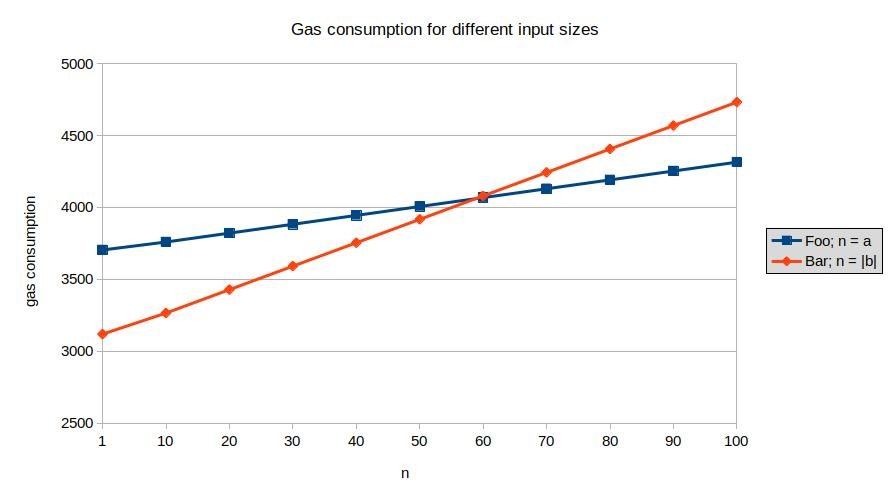
\includegraphics[width=0.9\linewidth]{figures/2-use_cases/cost_analysis}
\caption{Gas consumption of transactions calling \texttt{Foo} and \texttt{Bar} for increasing input sizes}
\label{fig:use_case_cost}
%\vspace{128in}
\end{figure}

Besides inflicting higher transaction costs on the user with increasing parameter sizes, a local approach also causes a higher ``footprint'' on the blockchain network. The transaction has to be processed at every full node of the network, which do not get any rewards in return (except for the nodes that were assigned baking or endorsement rights for the current block\footnote{Tezos' Proof of Stake consensus mechanism is described in \secref{sec:tezos}}).

    \externaldocument{1-introduction}

\chapter{Generic Offline Design}\label{chap:offline}
The implementation of distributed assertion checking on any blockchain requires some off-chain considerations and infrastructure. The previous chapter defined a formal set of logical formulae amenable for this approach and gave some in-depth examples. As stated before, the proposed implementation in the following chapters is, for the most part, restricted to formulas of predicate logic using universal quantification.\\
The purpose of the offline infrastructure is to provide a syntax for stating assertions that check logical formulas, as well as a toolchain to compile these assertions into code that can be originated on the target blockchain. Depending on the individual solution for the respective blockchain protocol, this can either be the original contract extended directly with the assertion code, or as a separate contract that extends the original contract in some other way. This chapter describes the generic part of the offline design, which corresponds to the front-end of the compilation pipeline shown in \figref{fig:pipeline_frontend}. As a start, \secref{sec:syntax} describes the concrete syntax for writing assertions and shows how it expresses some of the previously given examples. The transformation of the original assertions to assertions that check for counterexamples is formalized in \secref{sec:transformation}. Lastly, \secref{sec:accuracy} analyses the reliability of distributed assertion checking as proposed and the cost incurred by increasing it.

\begin{figure}[h]
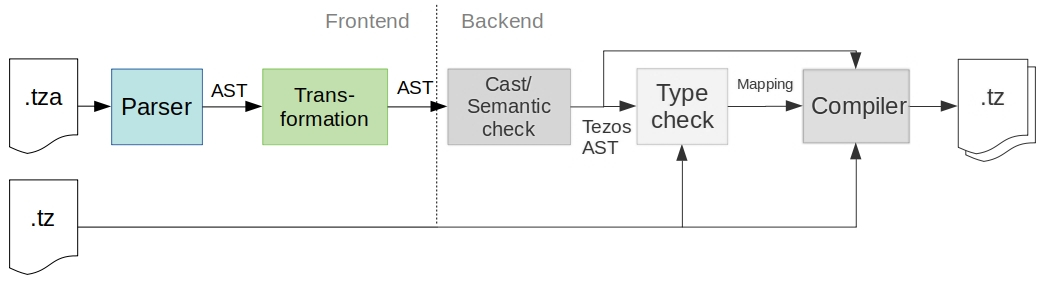
\includegraphics[width=\linewidth]{figures/3-offline/pipeline_frontend}
\caption{The stages of the generic frontend of the compilation pipeline}
\label{fig:pipeline_frontend}
\end{figure}

\section{Assertion syntax}\label{sec:syntax}
The assertion syntax is described in two versions by the EBNF grammars shown in appendix \ref{apx:grammar}. One version implements a prefix and the other one an infix notation. The pipeline currently supports the prefix notation with mandatory parentheses to avoid the need of handling operator precedences. To avoid context switches (at least for developers on Tezos), the assertion syntax references those of OCaml and thereby also Michelson.\\
A file containing assertions (henceforth referred to as ``assertion contract'') contains at least one assertion for some function or entrypoint of the original contract (henceforth referred to as ``parent contract''). An assertion begins with a signature consisting of an optional tag followed by a parameter type declaration. The tag can be used for documentation, but may sometimes be needed to indicate to which function of the parent contract the assertion should be assigned. The body is an (optional) nesting of quantifiers and conditions around exactly one assertion. Conditionals can be used to restrict the quantification domains or for some other constraints. For completeness, the existential quantifier is already included in the grammar, however the current version of the pipeline will reject any assertions containing it. \\
In order to make the front-end generic, the assertion grammar constitutes a union of operations and types for the target languages. This also allows the transformation to be oblivious of the target platform and be identical for all backends. The current version of the grammar recognizes all types present in the Tezos VM and a subset of operations that Michelson provides ( \secref{sec:tezos} contains an introduction to Tezos and Michelson and goes more into detail about this). Responsible for rejecting any assertions containing unsupported types or operations are the respective backends.\\

As an example, consider a variation of the formula given in \eqref{eq:sorted} that checks whether a given list is sorted in ascending order:
\begin{equation}\label{eq:sorted_v2}
	(\forall n : int)(\forall m : int) (0 \leq n < m < |a|) \Rightarrow a[n] \leq a[m]
\end{equation}
The respective assertion that checks this property for the parent contract from \lstref{lst:sorted} could be expressed as follows:
\lstinputlisting[caption=Assertion contract for checking if a list is sorted, language=Assertion, label={lst:sorted_assertion}]{listings/sorted.tza}

\subsection{Extensions}
In future iterations, the assertion syntax could be extended with some more features to improve usability and readability:
\begin{itemize}
\item \textbf{Local variables} to store, reuse and denominate computed values
\item \textbf{User-defined functions} to extract whole routines that can be reused in a single or even many assertion contracts, if defined as a module.
\item \textbf{if-else conditions} to adapt the domains of quantifications if certain conditions hold. The assertion that checks whether two numbers are relatively prime (discussed in \secref{sec:coprime}) is a good use-case for this feature: Firstly, the minimum of the given number has to be determined, however the \texttt{min}-function might not be supported as a built-in function by the target language (Tezos, for instance, does not support it). A solution for that could be to implement two branches in the program to handle each case. Secondly, if the greater of the two numbers is not evenly divided by the smaller one, the formula can be optimized by reducing the quantification domain by half to $(2 \le n \le \lfloor \frac{min(a,b)}{2} \rfloor)$, as a number cannot be evenly divided by any number between itself and its half \cite{bernhardt_veigel_2020}. With a syntax supporting an \texttt{if-else} control structure, the optimized assertion could look as follows:
\lstinputlisting[caption=Assertion syntax with if-else structures \cite{bernhardt_veigel_2020}, language=Assertion, label={lst:coprime}]{listings/coprime_ifelse.tza}
This feature is not included in the current version, because conditional domain restrictions make the translation from quantifiers to random generators or loops more complex. Aside from that, without the feature of variables and user-defined functions, the code is inflated significantly, thus causing increased origination cost.
\end{itemize}

\section{Transformation}\label{sec:transformation}
Since the validators will check the input parameter for the negation of the formula, it has to be transformed before compilation. Furthermore, the formula should explicitly state the domain for each quantifier, which will have to be translated into a set of bounds that refer to the respective random generator. Restricting the ranges of the random generators is important in order to avoid wasting resources through testing values out of the relevant (or legal) scope.

\subsection{Negation}
The formula is negated using the negation rules of second-order logic and applying De Morgan's laws \cite{de_morgan} until the negation is applied to the literals. Negating universal quantification is equivalent to an existential quantification of its negated body (and vice versa): $\neg \forall x P(x) \equiv \exists x \neg P(x)$ \cite{Sundstrom2020Quantifiers}. The domain restrictions are not affected by the negation, which is also reflected in the rules of predicate logic if the domain is given as a premise in the logical formula: $\neg (p \Rightarrow q) \equiv p \Rightarrow \neg q $.

\subsection{Building smart random generators}
In order to assign each explicit bound to its appropriate quantifier, the formula has be skimmed for atomic constraints that contain predicate (bound) variables. They're then moved and assigned to the quantifier that bounds the variable. If the constraint contains more than one bound variable, it is assigned to the quantifier with the highest depth in the order of quantifiers, as they depend on the generated value(s) of the other variable(s). \\
Revisiting the formula from \eqref{eq:sorted_v2}, its premise can be considered as a conjunction of the four constraints
\begin{itemize}
\itemsep-1em
\item $0 \leq n$
\item $n < |a| $
\item $n \le m$ and
\item $m < |a|$.
\end{itemize}
Applying the rules given above after negating the formula, the constraints are assigned to the quantifiers as follows:
\begin{equation}\label{eq:sorted_v2_bounds}
	(\exists n : int, 0 \leq n \wedge n < |a|])(\exists m : int, m > n \wedge m < |a|) \text{ } a[n] > a[m]
\end{equation}
Ultimately, the quantifiers are then translated to the corresponding random generators as indicated in \lstref{lst:rand}.
\begin{lstlisting}[label=lst:rand]
n = random(0, size(list))
m = random(n, size(list))
\end{lstlisting}
While conjunctions can be handled easily, other operators make it more difficult to derive efficient random generators. Consider the following constraints:
\begin{itemize}
\itemsep-0.7em
\item[1)] $(\forall n : int) (n < 10 \lor n > 20) ...$
\item[2)] $(\forall n : int) (n \ne 10) ...$
\item[3)] $(\forall n : int) (n = 10) ...$
\end{itemize}
Constraint 1) complicates restricting the random generator in several ways. Firstly, it separates the domain into two disjoint sub-domains, which requires defining a random generator for each range and another one to decide which one is called. Secondly, the operands of a disjunction cannot be considered separately when more than one bound variable is involved. For the predicate variable whose random generator is executed first, the domain restriction is optional, while the generation of the following random values depend on the previous result. Similarly to 1), constraint 2) splits the domain into sub-domains. To keep it simple for the time being, restrictions formulated with these operators are kept as part of the assertion code rather than used as constraints for the generators. Consequently, some validators may generate irrelevant values when checking the assertion and, depending on the size of the gap between the sub-domains, this can significantly decrease the reliability of this kind of assertion checking. Thus, further developed iterations should handle and translate them accordingly.\\
Constraint 3) effectively makes the quantifier, which binds $n$, obsolete. Adding this constraint to the respective generator will at least not affect the reliability, but a future improvement could be to optimize the assertion by replacing all occurrences of the bound variable with the assigned value and removing the quantification.

\subsection{Implicit constraints}
In some cases, boundaries are imposed implicitly by data types. List indices, for instance, are always bound to the range $0.. size(list) - 1$ and could thus be derived from the formula without an explicit specification. As this deduction makes the transformation more complex, requiring a semantic analysis of the formula, a completely explicit formula in terms of the domain is required for now. Depending on the VM, the lower bound for indexing operations can be implicitly handled by the random generator of an appropriate predicate type. As an example, Michelson supports the data type \texttt{nat} representing the natural numbers, which categorically excludes all values below zero. Developers aware of this can exploit this and, for instance, abbreviate \eqref{eq:sorted_v2} with the following formula:
\begin{equation}\label{eq:sorted_v2_abbr}
	(\forall n : nat)(\forall m : nat) (n \le m < |a|) \Rightarrow a[n] \leq a[m]
\end{equation}

\section{Accuracy of the approach}\label{sec:accuracy}
Since the proposed approach implements a probabilistic test, the accuracy as well as the costs incurred by guaranteeing a specified certainty threshold, need to be examined closely. The goal is to identify a formula that, given the domain of a formula in predicate logic, returns an estimate of a lower bound of samples necessary to find an existing counterexample with a probability $p$. From this analysis, it can be derived how effective a formula can be checked on a blockchain with $m$ validators. Sections \ref{sec:coupon} and \ref{sec:prob_threshold} depict the findings from \cite{bernhardt_veigel_2020} and are based on the assumptions that the random generator picks elements independently from a uniform distribution and that there exists exactly one counterexample for the passed parameter.

\subsection{Coupon Collector's Problem Analysis}\label{sec:coupon}
When checking properties with probabilistic testing, the result is either definitely not satisfied, or probably satisfied. Thus, errors only occur as false positives. In order to find an existing counterexample with probability $p = 1$, every element in the given domain $\mathcal{D}$ has to be checked by at least one validator. Deterministically, this is reachable with exactly $|\mathcal{D}|$ test runs. This is, however, invalid for the probabilistic approach, as some validators may generate duplicate random values and leave some elements of $\mathcal{D}$ unchecked. \\
In probability theory, this is known as the Coupon Collector's Problem \cite{croucher_collecting_2006}. Given $n = |\mathcal{D}|$, the probability that no duplicate elements are generated with $n$ picks is given by
\begin{equation*}
    p = \prod_{i=1}^{n} \frac{i}{n}
\end{equation*}
As an example, the probability that all validators generate a unique random value already drops to $0.036\%$ for $n = 10$. Let the random variable $T$ be the number of test runs executed until every element in the domain has been generated. In order to obtain an estimation of how many test runs are needed to find the counterexample for certain, the goal is to identify its expectation $E(T)$. To this end, the geometric probability distribution is applied \cite{croucher_collecting_2006}:\\
Each element is generated with a probability of $1/n$. Thus, the probability to generate the $i$th unique element is given by 
\begin{equation}
    p_i = \frac{n-i+1}{n}
\end{equation}
\cite{croucher_collecting_2006}. The expected value of a random variable $X$ is given by $E(X) = \frac{1}{p}$\cite{croucher_collecting_2006}, thus the expected number of test runs for $n$ is 
\begin{equation}
E(T) = n \sum_{i=1}^{n} \frac{1}{i}
\end{equation}
\tabref{tab:prob_outcomes} shows the expected number of test runs $E(T)$ and its standard deviation $\sigma$ for different $n$. Furthermore, $E(T)$ and $\sigma$ are used to calculate a 95\% confidence interval for $T$ by applying the central limit theorem, which provides an upper and lower bound on the number of test runs \cite{croucher_collecting_2006}. Rounded values for both bounds are also shown in \tabref{tab:prob_outcomes}.
\begin{table}[h]
    \centering
    \begin{tabular}{lllll}
        \thead{$n$} & \thead{$E(T)$} & \thead{$\sigma$} & \thead{lower bound} & \thead{upper bound}\\ \hline
        5 & 11.4 & 2.53 & 6 & 16\\
        10 & 29.3 & 4.32 & 21 & 38\\
        20 & 72.0 & 7.21 & 58 & 86\\
        30 & 119.8 & 9.48 & 101 & 138 \\
        50 & 225.0 & 13.23 & 199 & 251 
    \end{tabular}
    \caption{Expectation, standard deviation and upper and lower bound of needed test runs for some $n$ \cite{croucher_collecting_2006}}
    \label{tab:prob_outcomes}
\end{table}

The results show that checking random values is a very inefficient approach if false positives are not admissible. Even if the lower bound of $T$ is chosen as the number of test runs, it exceeds the size of the domain by far and increases the time complexity to $\mathcal{O}(n*log(n))$ for large $n$ \cite{xu_tang_2011}. For instances where false positives are tolerable, the following section introduces a formula to calculate the number of test runs that detect counterexamples with a given probability threshold $p \leq 1$.

\subsection{Setting probability thresholds}\label{sec:prob_threshold}
The goal is to find a number $t$ of test runs, s.t. the probability $P_{c,t}$ of not finding the counterexample drops below a certain threshold $c$. A validator finds the counterexample in one test run with probability $\frac{1}{n}$, and misses it with probability $(1-\frac{1}{n})$. After $t$ tests runs, the probability that the counterexample has not been found is thus $(1-\frac{1}{n})^t$. Following the same approach as in \cite{mahl_schindel_2007} to retrieve an upper bound for $P_{c,t}$, we use the following inequality
\begin{equation}
(1-\frac{1}{m})^m \leq \frac{1}{e}
\end{equation}
which holds for all $m > 0$. From this inequality, it follows that
\begin{equation}
(1-\frac{1}{n})^t = ((1-\frac{1}{n})^n)^{\frac{t}{n}} \le e^{-\frac{t}{n}}
\end{equation}
With this, the probability $P_{c,t}$ of not finding the counterexample with $t$ test runs can be defined as
\begin{equation}
P_{c,t} \le e^{-\frac{t}{n}}
\end{equation}
In order to retrieve the number of test runs $t$ necessary for $P_{c,t}$ to drop below a specified threshold $c$, the inequality is solved for $t$, which is then dependent of the known parameter $n$ and an arbitrary value for $c$:
\begin{align}
    e^{-\frac{t}{n}} &\leq c && \text{with } 0 \leq c\le 1 \nonumber\\
    t &\geq -n\:\ln(c)
\end{align}
For $c = \frac{1}{e}$ ($\approx 36.79\:\%$) the lower bound of $t$ is exactly $n$, which means that for higher reliabilities the number of test runs needs to be greater than $n$. \figref{fig:graph_t_c} shows the lower bounds of $t$ as a function of the probability threshold and domain size. One can see that the increase in accuracy is approximately linear to the number of test runs below a threshold of $c=0.5$, but requires an exponential testing effort to reach higher thresholds.
\begin{figure}[h]
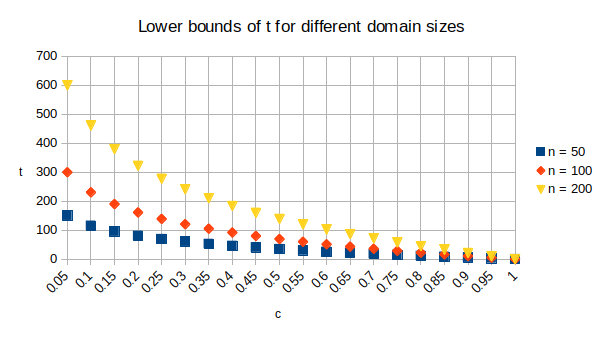
\includegraphics[width=0.95\linewidth]{figures/3-offline/graph_t_c}
\caption{The number of required test runs as a function of the probability of false positives $c$ and size of the domain $n$}
\label{fig:graph_t_c}
\end{figure}
For assertions with several quantifiers, which are translated to random generators, all domains have to be considered in the calculation. Revisiting the intersection of sets from \secref{sec:existential}, every element in set $U$ has to be compared to every element in set $V$. Thus, the lower bound of test runs needed to check whether they intersect with a certainty of 63.21\% is given by $t \leq t_1 * t_2$ with $t_1 \geq |U|$ and $t_2 \geq |V|$.

\subsection{Validators vs. test runs}
The last section derived a formula to calculate a lower bound for a number of test runs $t$ in order to reach a certain level of confidence. However, $t$ is not a parameter that can be adjusted to an arbitrary value on the blockchain, as the assertion is checked by the validators. Assuming a blockchain has $m$ validators, the actual lower bound of test runs is $m$. For cases where there are not enough validators to reach a threshold $c$, a mechanism is required to have each validator check the property for multiple random values. Hence, the actual executed number of checks is always a multiple of $m$. \secref{} goes into a bit more detail about this based on the Tezos blockchain. \todo{Refer to section}

\subsection{Alternatives to random testing}
For applications where higher reliability is crucial, an alternative to checking elements randomly could be to coordinate a systematic iteration of the domain. The implementation of such a coordination is not trivial though; validators can't simply be passed an individual value as input. Instead, possible approaches could be to implement a central instance that allocates an element in the search space to each validator, or use some unique and intrinsic attribute, like an identification number, as input for a mapping. The discussion if this approach would provide any advantages over a local validation of the property is left open \todo{Depends on cost analysis?}.

\subsubsection{Central instance assigning values}
For this approach, the tool-chain would need to generate a separate contract that is called by the miners and validators as a proxy. This contract would then, for instance, generate a number using a modulo-n counter and pass this number as an additional parameter to the assertion code. The random generators would be omitted accordingly. However, this works only as expected if there are no simultaneous transactions calling the contract, otherwise it cannot be guaranteed that all elements have been checked for each of the transactions. If and how this issue can be solved will not be discussed further in this thesis.

\subsubsection{Using unique attributes of a validator}\label{sec:alt_attributes}
This approach strongly depends on whether the validators have a unique id or other attribute that can be accessed from within a contract.  If there is (or the language can be extended with such a feature), there needs to exist a non-injective surjective function that maps the respective attributes represented by type A to an element of the domain represented by type B, i.e. $f: X \rightarrow Y$. Furthermore, for cases where $t > m$, an offset needs to be added, s.t. a validator checks distinct elements for each test run. \\
Implementing such an approach on Tezos becomes even more challenging due the way endorsing (i.e. validation) rights are distributed in its proof-of-stake mechanism: for each block level, endorsing rights are assigned to the owner of a randomly selected roll, i.e., a set of tokens \cite{tezos_docs}. This means that the same validator can be picked multiple times for endorsing one block and thus some elements in the domain may remain unchecked. \secref{} goes into more detail about this issue. \todo{Ref section}
    \chapter{Tezos-specific Offline Design}\label{chap:offline_tezos}
After parsing an assertion contract and transforming it, the resulting AST is passed to the target-specific backend. For this thesis, the platform target is Tezos, with Michelson as the compilation target. This chapter continues to describe the pipeline stages implemented in the Tezos backend, which are shown in \figref{fig:pipeline_backend}. Furthermore, it states the necessary extensions to Michelson and its evaluator to facilitate useful assertions using random generators and assesses several orchestration strategies between the parent and assertion contract code. As a preliminary, the following section gives a short introduction to the Tezos blockchain, the Michelson language and some relevant tools in Tezos' ecosystem.

\section{Introduction to Tezos}\label{sec:tezos}
The Tezos blockchain is presented in its whitepaper as a \enquote{generic and self-amending crypto-ledger} \cite{goodman_tezos_2014}. It uses a proof-of-stake consensus mechanism that is not only used to agree on the current state of its ledger, but also allows its stakeholders to come to a consensus about changes in the economic protocol by participating in a voting process. The changes included in a protocol upgrade, called amendment, can influence i.a. which transactions are valid on the blockchain, the payment system or even the voting process itself without risking a fork of the blockchain. Everyone owning the cryptocurrency of Tezos, called Tez, is considered a stakeholder and can participate in the consensus mechanism. The whitepaper compares the self-amending protocol of Tezos to a game created by Philosopher Peter Suber called ``Nomic'', whose set of rules are subjected to a democratic voting system \cite{nomic}. Similar concepts can also be found in modern pop culture, such as the virtual sports league ``Blaseball'' \cite{blaseball} that became popular during the COVID-19 pandemic.

In addition to user accounts associated with a public key, Tezos supports smart contracts, which are written in the built-in language Michelson. Tezos' transaction fee system is similar to that of Ethereum \cite{wood_ethereum_2021} - it is gas-instrumented and besides a base fee, every operation and byte of storage during contract execution has to be paid for. However, Tezos imposes a hard cap on the amount of gas that can be consumed per operation (including internal transactions) \cite{tezos_docs}\cite{morley_repo}, whereas Ethereum limits the gas quota only in respect to blocks \cite{wood_ethereum_2021}.\\
Tezos is written in the multi-paradigm programming language OCaml \cite{ocaml_doc}. Compiling the its source code yields five essential binaries: the node, baker, endorser, accuser and client. The node is the entity that connects to the peer-to-peer network and keeps a copy of the chain. Bakers are responsible for producing new blocks, the endorsers for validating new blocks and the accusers to call out bakers or endorsers which double-sign or -endorse. The client provides a command line interface to interact with the local node through remote procedure calls (RPC).

\subsection{Proof-of-stake in Tezos}
In Tezos, contracts that staked a minimum amount of tokens, called a roll, can participate in the consensus mechanism and can either have the role of a baker or endorser. Contracts who don't own enough tokens or infrastructure to participate directly can delegate their baking and endorsing rights to other contracts. The rights are determined and assigned at the beginning of each cycle, which consists of a specified number of blocks. For baking, a random roll is selected for each block level and the rights are assigned to its owner. The block produced by that baker is endorsed by a fixed number of endorsers (currently 32 in protocol 008 Edo), which also have been assigned endorsing rights for this block level by a random selection of rolls. Since participants can stake more than one roll, an endorser may be assigned several endorsement slots at the same block level. \\
As an incentive for active participation in the consensus algorithm, delegates (and also delegators) receive rewards in form of tokens. However, if accusers detect double-baking or -endorsement, the delegate is penalized by burning (i.e., destroying) their security deposit. \cite{tezos_docs}

\todo{Add mempool? If Blockchain protocol is outlined}

\subsection{Michelson}
Michelson is a lower-level, stack-based language with strict type-checking and supports primitive data types, like integers or strings, as well as high-level data structures such as list, maps and sum types \cite{tezos_docs}. The type system reduces the occurrence of runtime errors and ensures that only well-typed contracts are originated on the blockchain. \\
The concrete syntax of Michelson is called Micheline. A program is represented in Micheline nodes, which can be one of the following constructs:
\begin{itemize}
\item A constant of type integer (in decimal notation)
\item A constant of type string
\item A byte sequence in hexadecimal notation
\item An application of a language primitive to a sequence of nodes
\item A sequence of nodes
\end{itemize}
For documentation, readability and additional type constraints, Michelson and Micheline also offer three types of annotations - type, variable and field or constructor annotations, which are labelled with a unique special character in Micheline. The toplevel structure of a smart contract consists of a sequence of the three primitives \texttt{parameter, storage} and \texttt{code}, declaring the type of the input parameter, the storage type and the actual program code. The full grammar of Micheline and Michelson can be found in the Tezos developer resources \cite{tezos_docs}.

\subsubsection{Entrypoints}
Unlike the contracts shown so far, which were expressed with the syntax of Ethereum's contract language Solidity \cite{solidity_docs}, Michelson doesn't have a concept of named functions with individual input parameter types. Instead of named functions, Michelson programs can have separate entrypoints by taking a disjunctive type as input parameter and optionally tagging the type constructors with a "function" name. The disjunctive type is built by nesting the \texttt{or} type, which has the constructors \texttt{left} and \texttt{right}. Assume we want to implement the contract from \lstref{lst:prime} in Michelson and add another function to it, which expects a string parameter. Omitting the actual program, the contract type declaration looks as follows:
\begin{lstlisting}[language=Michelson, numbers=none, caption=Michelson contract with two entrypoints, label=lst:entrypoints]
parameter (or (int %isPrime) (string %isUpper));
storage unit;
code {
  ...
  IF_LEFT { ... (* then *)}
          { ... (* else *)}
}
\end{lstlisting}
The input type declared in the primitive application \texttt{parameter} accepts input of either type \texttt{left int}, or \texttt{right string}. By adding the field annotations \texttt{isPrime} and \texttt{isUpper}, the entrypoints are given tags and can be called explicitly by an external transaction. In that case, parameters of type \texttt{int} or \texttt{string} are accepted and the value is automatically wrapped into the respective constructors. Furthermore, it's possible to declare a \texttt{default} entrypoint, which is called when no explicit tag is specified. By default, the default entrypoint is assigned to the root of the parameter type. \cite{tezos_docs}

\subsubsection{Internal operations}
Smart contracts are able to call other smart contracts by emitting internal operations. The return type of Michelson programs is a tuple of a list of internal operations and the updated storage. Thus, after the actual contract has been executed, the operations of the returned list are run in sequence. Since the internal operations may in turn also emit internal operations, they are put into a queue and are processed in order. As an example, \figref{fig:internal_ops} shows an execution order of two external transactions, i.e., transactions which have been initiated by a user account, and their internal operations.
\begin{figure}[h]
\centering
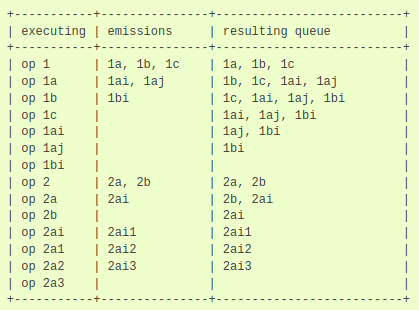
\includegraphics[width=0.5\linewidth]{figures/4-offline_tezos/internal_ops}
\caption{Execution order of two external operations and their internal operations; Source: \cite{tezos_docs}}
\label{fig:internal_ops}
\end{figure}

Both external and internal operations can fail if the source does not have enough balance to spend the specified amount, a gas limit was reached or if a program fails when reaching a \texttt{FAILWITH} instruction. If a failure occurs, the whole sequence fails and all changes up to the point of failure are reverted.

\subsection{Developer tools in the Tezos ecosystem}
This section describes some relevant tools and projects for developers that are part of Tezos' ecosystem.

\subsubsection{Tezos Libraries}
Tezos' executables and libraries are developed in the programming language OCaml and are available on through OCaml's package manager \texttt{opam} \cite{tezos_opam}. The protocol libraries of every version are released separately, thus any projects can be built on the protocol of choice. Important libraries that were used in the development of the offline toolchain are the Micheline library providing the internal abstract syntax tree (AST) and parser of the Michelson language, as well as the protocol specific libraries containing i.a. the type checker. Additionally, the client libraries are used to retrieve any needed information from the node or blockchain via RPCs.

\subsubsection{Testing tools}
Before a new protocol is proposed to the Tezos network, it has to be thoroughly tested with system, integration and regression tests. This requires a sandboxed network to simulate the real peer-to-peer network, such that also interactions between the actors of the blockchain can be tested. Tezos' development environment provides two testing frameworks for this:
\begin{itemize}
\item[\textbf{Flextesa}] With Flextesa (Flexible network sandboxes)\cite{tezos_docs} one can configure and run a small, fully functional sandboxed test network including nodes, bakers, endorsers and accusers. Accounts can be instantiated and used to send or receive funds. Configurable are, for instance, the size of the network, the time between blocks or enabling generation of random network traffic. Networks may either be fully autonomous, baking blocks automatically, or require manual baking of blocks. It also supports interactive sessions, where the tester can interact with the blockchain using the Tezos client. Flextesa's typical use-cases are interactive testing scenarios like double-baking, the voting process or protocol amendments. The Tezos repository already provides ready-to-use scenarios for accusations. Besides testing shell or protocol code, Flextesa can also be used to test smart contracts.
\item[\textbf{Tezt}] The Tezt framework \cite{tezos_docs} is newer than Flextesa and planned as its replacement. It launches the Tezos binaries as external processes to build a sandboxed test network of configurable size. Its main advantages over Flextesa are simplicity, better usability and extendibility and better performance due to the use of an event system instead of polling the node.
\end{itemize}

\subsubsection{High-level languages}
Michelson is a compilation target for various high-level languages that provide a more user-friendly and intuitive way of writing smart contracts. Additionally, some of them come with development environments and testing or verification tools. The following list comprises of the three most prominent languages that compile to Michelson:
\begin{itemize}
\item[\textbf{Liquidity}] \cite{liquidity} is a language with an OCaml-like syntax, which allows using local variables instead of stack manipulations. Its module system can be used to write reusable contract code or libraries. Besides an optimizing compiler, the project also includes a decompiler to compile Michelson programs to Liquidity.
\item[\textbf{SmartPy}] \cite{smartpy} is a language available through a Python library and lets developers write contracts and tests using Python syntax and structures (such as classes). Its developer suite includes i.a. a compiler, a simulation engine for testing contracts and an online editor.
\item [\textbf{fi}] 's \cite{fi} syntax is similar to JavaScript or Ethereum's contract language Solidity. It also provides an online editor and a simulator to test against the compiled contracts. However, it seems extensions to Michelson introduced by newer protocol versions are not supported yet.
\end{itemize}

\section{Extensions to Michelson}
The way Michelson is interpreted is purely functional; it takes the current stack and an operation and builds a return stack from the initial one, without causing any side effects \cite{tezos_docs}. The recursive Michelson interpreter is defined as as a list of rules comprising of all possible inputs, i.e. program and stack types, and the respective output stack type of the computation if a rule applies. Each rule is of the following form: 
\begin{lstlisting}[caption=Rules form in the Michelson interpreter \cite{tezos_docs}, language=, numbers=none, label=lst:rules]
> (syntax pattern) / (initial stack pattern)  =>  (result stack pattern)
    iff (conditions)
    where (recursions)
    and (more recursions)
\end{lstlisting}
For each valid program and initial stack exactly one rule matches (given that any extra conditions over values on the stack, stated after the \texttt{iff} keyword are true) \cite{tezos_docs}. If the result depends on the results of other program interpretations (given after the keywords \texttt{iff, where, and} in rule form), the rule only applies if these partial results also match the respective intermediate result stack patterns.\\
In addition, there exists a typing rule for each syntax construct that restricts the valid input stacks. The typing rules use the meta variables \texttt{'a} for type and \texttt{'A} for stack type variables in order to express consistency within the program (not polymorphism). These rules are given in the following form:
\begin{lstlisting}[caption=Form of typing rules in Michelson's specification \cite{tezos_docs}, language=, numbers=none, label=lst:type_rules]
(syntax pattern)
:: (type of stack before) -> (type of stack after) [rule-name]
   iff (premises)
\end{lstlisting}
The type notations, as well as syntax and stack patterns are listed in \cite{tezos_docs}.

Since Michelson is implemented in the protocol-specific part of the blockchain code, adding new instructions require a protocol update. The instruction must be added i.a. to the list of tokens, its computation to the interpreter and its typing rules to the type checker. As the computation of the new instruction must be paid for like any other instruction, the protocol must also specify a gas cost. Previous extensions to the Michelson language, such as \cite{tezos_michelson_ext}, can be used as a guideline for the implementation and the gas cost specification in \cite{tezos_repo_gas} as an orientation to how high the gas costs should be scheduled for comparable instructions.

From the given formulas and assertion examples so far, one can derive a set of necessary instructions that need be be present in the target language. The following subsections list the instructions which have to be added to Michelson's instruction set, specify their selection and typing rules and describe how they can be implemented in the interpreter. These do not necessarily include high level instructions, like \texttt{sqrt} from \eqref{eq:prime}, that can be reproduced by using lower level instructions. For these purposes, a later iteration of the syntax will provide the feature of user-defined functions.

\subsection{Random}
A vital instruction that cannot be expressed with Michelson's current instruction set (state of protocol 008 Edo \cite{tezos_docs}) is the generation of a random value of certain types. Since smart contracts need to be deterministic, s.t. the network can reach a consensus about the state of the ledger \cite{chatterjee_probabilistic_2019}, the prevalent workarounds for generating pseudo-random numbers cannot be used for assertion checking. Distributed assertion checking explicitly requires as many validators as possible to generate a unique value, whereas common schemes for randomness, like oracles or using block attributes as seeds \cite{chatterjee_probabilistic_2019}, will provide the same values for all validators.\\
\lstref{lst:rand_type} specifies the selection and typing rule of a new instruction \texttt{rand}, which consumes an offset and a positive range from the stack and pushes a randomly generated integer to the top. This instruction, of course, can also be provided for other data types, such as \texttt{nat}, \texttt{string} or \texttt{mutez}.
\lstset{upquote=true}
\begin{lstlisting}[caption=Selection and typing rules of the integer \texttt{rand} instruction, language=, numbers=none, label=lst:rand_type]
:: int : nat: 'A -> int : 'A
> RAND/ offset : range : S  => int : S
\end{lstlisting}

Within the Michelson interpreter, the selection of rules is implemented as a huge match case \cite{tezos_repo}. If the rule for \texttt{rand} applies, the respective computation in OCaml could look as drafted in \lstref{lst:rand_impl}.
\begin{lstlisting}[caption=Simplified evaluation of \texttt{rand} in the Michelson interpreter, language=, label=lst:rand_impl]
match (instruction, stack) with
...
| (Rand (offset, (range, rest))) -> 
   Random.self_init;
   let rand_int = offset + Random.int(range) in
   return (rand_int, rest)  (* Resulting stack *)
\end{lstlisting}

\subsection{Nth}
An exception for not adding higher level instructions may be the more fundamental operation \texttt{nth} for accessing list elements, as it is used (sometimes more than once, ref. \eqref{eq:sorted_v2}) in many use cases. Adding an own predefined primitive for this reduces the origination costs of the assertion contract, given that its equivalent in the current instruction set requires the compiler to generate a workaround using iteration, for instance a loop or list iterator. As a first approximation, appendix \ref{apx:nth} shows a potential implementation of \texttt{nth} in Liquidity (\lstref{lst:nth_liq}) using a loop, and how the respective Michelson code looks like after compiling the contract with the Liquidity compiler (\lstref{lst:nth_tz}). \\
In case the \texttt{nth} is added as a predefined primitive to Michelson for the type \texttt{'a list}, its selection and typing rules are specified as follows:
\begin{lstlisting}[caption=Selection and type rule of the list \texttt{nth} instruction, language=, label=lst:nth_type]
:: (list 'a) : nat : 'A -> option 'a : 'A
> NTH / l : index : S  =>  Some 'a: S
     iff index is within bounds
> NTH / l : index : S  =>  None 'a: S
     iff index is out of  bounds
\end{lstlisting}
As Michelson lists are represented with OCamls list type within the VM \cite{tezos_repo}, the computation for \texttt{nth} could look as shown in \lstref{lst:nth_impl}.
\begin{lstlisting}[caption=Simplified evaluation of \texttt{nth} in the Michelson interpreter, language=, label=lst:nth_impl]
match (instruction, stack) with
...
| (Nth ({elements = []; _}, (_, rest))) ->
  return ((None, rest)
| (Nth ({elements = es; length}, (index, rest))) ->
  let l_length = of_int length in
  if index <= l_length
    then return (Some (List.nth es index), rest)
    else return (None, rest)
\end{lstlisting}
\lstset{upquote=false}

\subsection{failwith 2.0}
\draft{}
- failwith returns a failure string
- assertion execution -> random number is generated
- if counterexample is found, the random number somehow has to be extracted from the contract execution, s.t. other validators can verify the counterexample
- some special failure operation may be needed that returns the that value
- as representation of a counterexample is still an open question, there are not specifics yet as to how this instruction is supposed to look like (or if it is needed at all)

\section{Orchestration of contract and assertions}
So far, the assertion and parent contract have been considered separately. However, on the blockchain they have to be orchestrated, s.t. the bakers and validators execute the assertion before the actual contract code. The orchestration does not only include the linking of assertion and contract code, but also a mechanism to execute an assertion $t$ times depending on the domain space that needs to be checked. There are basically two approaches - the assertion and contract code can be assembled into a single monolithic contract, or they can be originated separately as standalone contracts. As the strategy has an impact on the compilation process and output, it has to be determined in advance which of the two should be implemented and how.

\subsection{Approach 1: Monolithic contract}
In the monolithic approach, a new contract is built using both the assertion and parent code as input. As is outlined in \figref{fig:monolithic_orchestration_basic}, the assertions can either be appended to the original contract as separate entrypoints or by prepending them to the code of the respective entrypoint. This tightly couples and unites the code in one self-contained unit.
\begin{figure}[!htb]
\subfloat[Appending assertions as separate entrypoints]{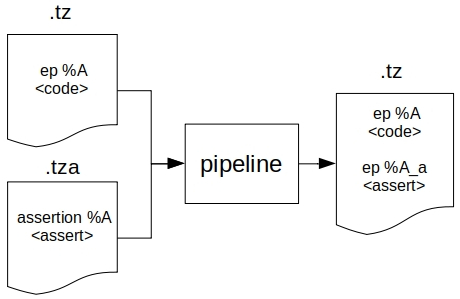
\includegraphics[width=0.5\textwidth]{figures/4-offline_tezos/pipeline_output_mono_ep_basic.jpg}}
\quad
\subfloat[Inserting the assertion code into the original entrypoint]{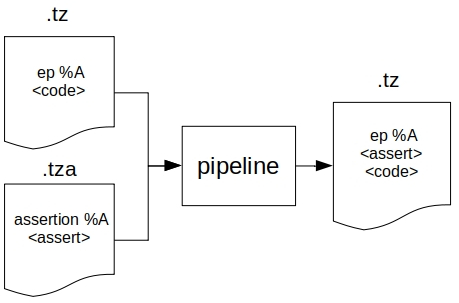
\includegraphics[width=0.5\textwidth]{figures/4-offline_tezos/pipeline_output_mono_basic.jpg}}
\caption{Approaches for assembling a monolithic contract}
\label{fig:monolithic_orchestration_basic}
\end{figure}
While the link between assertion and contract code is already given in a), the entrypoint and assertions in b) still need to be coupled, as it is not inherent which entrypoint represents a normal and which the respective assertion. For this reason, assertion entrypoints need to have fixed name pattern, s.t. it is derivable from the original entrypoint. As a proposal, the tag of the assertion is the tag of its parent entrypoint suffixed with a \texttt{\_a}, e.g. \texttt{A\_a} for entrypoint \texttt{A}. The baker can then execute the contract normally by calling the original entrypoint and prompt the validators to execute the assertion separately. \\
Both approaches, however, do not yet provide any means to have validators execute the assertions $t$ times. Since only the contract itself knows how to calculate $t$ (as per the range(s) of the random generator(s)), it cannot be passed to the validators as a parameter to the validation request. Instead, the contract itself needs a test run manager which handles this. A test run manager can either be implemented as another entrypoint, say \texttt{A\_m}, which then calls \texttt{A\_a} (or \texttt{A} in case of a)) $t$ times as an internal operation. Because transactions on Tezos guarantee either total success or total failure \cite{tezos_docs}, the execution is stopped as soon as one of the internal operation fails, i.e. detects a counterexample. When extending the diagram for a) with the manager, the pipeline output thus look as shown in \figref{fig:monolithic_orchestration}. The output for b) is analogue.
\begin{figure}[h]
\centering
  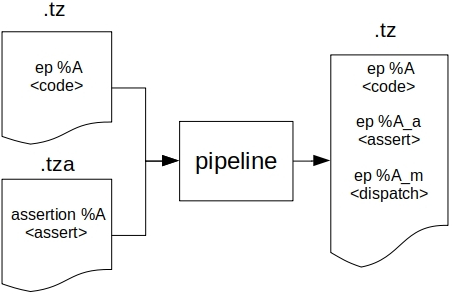
\includegraphics[width=0.5\textwidth]{figures/4-offline_tezos/pipeline_output_mono_ep.jpg}
	\caption{Monolithic assembly with separate entrypoints for manager and assertion}
	\label{fig:monolithic_orchestration}
\end{figure}
Another possibility is to create a separate manager contract that acts as a proxy, contains the manager code and internally calls the monolithic contract. This solution is a hybrid of the monolithic and modular approach. The section covering the modular approach describes in more detail how it is implemented.\\
It's important to realize that neither baker nor validators can differentiate between entrypoints that have an associated assertion and those that do not. In order to avoid transaction failures caused by calling assertions that do not exist, the compiler has to add dummy managers for empty assertions that call the actual contract code immediately. \lstref{lst:manager} drafts the manager code for entrypoints with and without assertions in pseudocode (assuming a purely monolithic implementation). 
\begin{lstlisting}[label=lst:manager, caption=Implementation of the manager in pseudocode]
%A (i : int) { ... }

%A_a (i : int) { .. assert (...) }

%A_m (i : int) {
	n = compute_n(i)
	Do m = 1 to n
		call(self, A_a, i)
}

%B (j : int) { ... }

%B_m (j : int) { call(self, B, j) }
\end{lstlisting}

\figref{fig:interaction_monolithic} and \ref{fig:interaction_monolithic_managertz} depict the interaction of the baker and validators with the resulting contracts on the blockchain for a variant using a single monolithic contract versus a hybrid solution. After calling a contract that includes an assertion, the baker has to keep the transaction in its mempool, a buffer where a node keeps prevalidated transactions not yet included in a block \todo{remove explanation if added to Tezos chapter}. Before it can be included, the transaction has to be kept there for a minimum amount of time, s.t. the validators have enough time to validate the assertion \todo{refer to blockchain protocol chapter if there is one}. The bakers therefore need to execute such transactions in a dedicated ``challenge'' mode, which could be signalled by using a special operation type to call such contracts. Operation types in Tezos are, i.a., transactions, originations or endorsements. By adding, for instance, a special transaction type (abbreviated by \texttt{txa} in the interaction diagrams), bakers can differentiate between normal transactions and those with assertions.
\begin{figure}[h]
\centering
  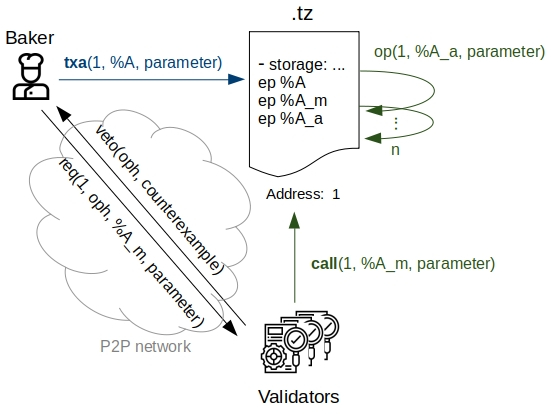
\includegraphics[width=0.7\textwidth]{figures/4-offline_tezos/interaction_monolithic.jpg}
	\caption{Interaction with a monolithic contract}
	\label{fig:interaction_monolithic}
\end{figure}

\begin{figure}[h]
\centering
  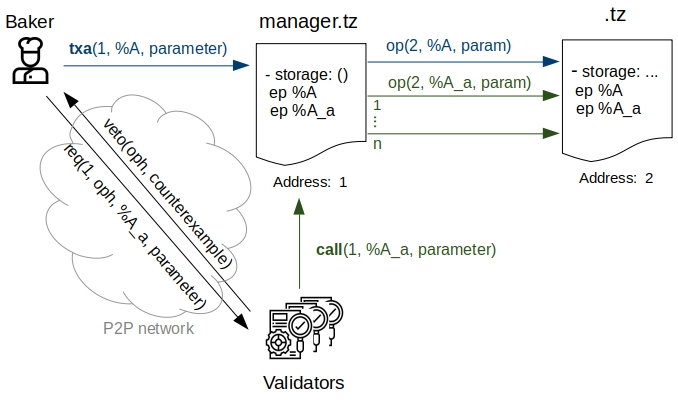
\includegraphics[width=0.8\textwidth]{figures/4-offline_tezos/interaction_monolithic_managertz.jpg}
	\caption{Interaction with a manager and monolithic contract}
	\label{fig:interaction_monolithic_managertz}
\end{figure}

After prevalidating a transaction in the challenge mode, the baker then sends a request to the network to check the associated assertion. The request contains the address of the monolithic contract or manager, the operation hash (oph) of the prevalidated transaction, the derived entrypoint tag of the assertion and the parameter. The operation hash is used to relate a counterexample to the respective transaction. Upon receiving such a request, the validators call the assertion manager; what type of operation is used for is an open question for the protocol design. For efficiency, at most the test runs detecting a counterexample should be recorded on the blockchain, which would not be the case if validators use standard transactions. What has been left out so far in the offline design is the representation of a counterexample. \secref{} briefly discusses this as an open question and follow-up of this thesis \todo{secref}.

\subsubsection{Evaluation of the monolithic approach}
The presented implementations of the monolithic approach each have strengths and weaknesses. Generally, they all share a pivotal disadvantage - they require a modification of the parent contract. This not only complicates the compilation process by requiring a decompilation of the parent code and an interweaving of the assertion code, but it also restricts the integration of assertions to contracts that have not yet been originated on the blockchain. \lstref{lst:mono} shows the skeleton of a monolithic contract that results from the given parent and assertion contract; both the parameter type and the branching of the code body have to be adapted. Another problem are contract invocations using the default entrypoint: firstly, the derivation of the entrypoint for the assertion becomes considerably more complex, as no explicit tag is given. Secondly, the parameter cannot be passed unmodified to the assertion, because the parameter types in respect to the default entry point do not match. For instance, invoking the default entrypoint of \texttt{example\_monolithic.tz} (\lstref{lst:mono}) with parameter \texttt{Left 4} calls \texttt{A}, but the respective assertion \texttt{A\_a} expects the value as \texttt{Left (Left 4)}. \\
Due to the tight coupling of parent and assertion code, this approach is also inflexible, since adaptions to either part require a recompilation and new origination of the whole code.
\lstinputlisting[label=lst:mono, caption=Skeleton of a monolithic contract in Michelson, numbers=left]{listings/monolithic.tz}

The distinct advantages and disadvantages of each combination of given implementation approaches are described briefly in the following matrix in \tabref{tab:mono_eval}.
\begin{table}[h]
	\centering
	\newcommand{\tabitem}{~~\llap{\textbullet}~~}
	\caption{Advantages and disadvantages of monolithic implementations}
	\label{tab:mono_eval}
	\subfloat[Monolithic w/ manager and assertion entrypoints] {
		\centering
		\begin{tabular}{ | p{0.5\linewidth} | p{0.5\linewidth} |}
		\hline
		\thead{Advantages} & \thead{Disadvantages} \\ \hline
		\begin{itemize}[leftmargin=*,noitemsep,topsep=0pt,parsep=0pt,partopsep=0pt]
		\item Contract and assertion can be called separately $\rightarrow$ parent code is only executed once
		\end{itemize} &
		\begin{itemize}[leftmargin=*, noitemsep,topsep=0pt,parsep=0pt,partopsep=0pt]
		\item More complex compilation; adds 1-2 entrypoints per native entrypoint
		\item Less readability
		\end{itemize} \\ \hline
		\end{tabular}
	}

	\subfloat[Monolithic w/ manager entrypoints and prepended assertion] {
		\centering
		\begin{tabular}{ | p{0.5\linewidth} | p{0.5\linewidth} |}
		\hline
		\thead{Advantages} & \thead{Disadvantages} \\ \hline
		\begin{itemize}[leftmargin=*, noitemsep,topsep=0pt,parsep=0pt,partopsep=0pt]
		\item Bypassing the assertion is not possible
		\end{itemize} &
		\begin{itemize}[leftmargin=*, noitemsep,topsep=0pt,parsep=0pt,partopsep=0pt]
		\item Cost inefficient - validators execute the assertion + code $t$ times
		\item Also only works with explicit entrypoint tags
		\end{itemize} \\ \hline
		\end{tabular}
	}

	\subfloat[Hybrid w/ manager and assertion entrypoints] {
		\centering
		\begin{tabular}{ | p{0.5\linewidth} | p{0.5\linewidth} |}
		\hline
		\thead{Advantages} & \thead{Disadvantages} \\ \hline
		\begin{itemize}[leftmargin=*, noitemsep,topsep=0pt,parsep=0pt,partopsep=0pt]
		\item Contract and assertion can be called separately
		\item Modularity $\rightarrow$ manager contract can be adapted independently
		\item Readability
		\end{itemize} &
		\begin{itemize}[leftmargin=*, noitemsep,topsep=0pt,parsep=0pt,partopsep=0pt]
		\item Higher initial origination costs due to more boilerplate code
		\end{itemize} \\ \hline
		\end{tabular}
	}

	\subfloat[Hybrid w/ manager entrypoints and prepended assertion] {
		\centering
		\begin{tabular}{ | p{0.5\linewidth} | p{0.5\linewidth} |}
		\hline
		\thead{Advantages} & \thead{Disadvantages} \\ \hline
		\begin{itemize}[leftmargin=*, noitemsep,topsep=0pt,parsep=0pt,partopsep=0pt]
		\item Bypassing the assertion is not possible
		\item Modularity
		\item Readability
		\end{itemize} &
		\begin{itemize}[leftmargin=*, noitemsep,topsep=0pt,parsep=0pt,partopsep=0pt]
		\item Cost inefficient - validators execute the assertion + code $t$ times
		\item Higher initial origination costs due to more boilerplate code
		\end{itemize} \\ \hline
		\end{tabular}
	}
\end{table}

\subsection{Approach 2: Modular contracts}\label{sec:modular}
With the modular approach, the assertion manager and each of the assertions are originated as separate contracts on the blockchain. The manager mirrors the interface of the parent contract, while each assertion each only has a single entrypoint which expects the raw parameter type. Due to the ``outsourcing'' of the assertion code, the parent contract remains pure and does not have to be modified. Similar to the hybrid solution from the last section, the manager calls the respective assertion contract $t$ times as an internal operation before calling the actual contract. In the case of empty assertions, it calls the parent contract immediately. Correspondingly, the pipeline outputs 1-$m$ contracts, where $m$ is the amount of entrypoints with an associated assertion, as depicted in \figref{fig:modular_assembly}.
\begin{figure}[h]
\centering
  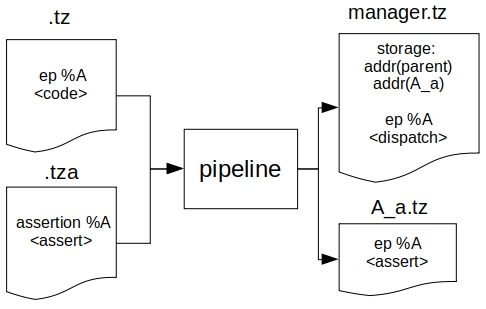
\includegraphics[width=0.6\textwidth]{figures/4-offline_tezos/pipeline_output_modular.jpg}
	\caption{Modular assembly of assertion and manager code}
	\label{fig:modular_assembly}
\end{figure}

In order to link the separate contracts to each other, the manager needs to know the addresses of the other contracts, which ultimately entails a fixed origination order. The independent assertion and parent contract(s) have been originated first, so that their addresses can be passed to the manager as initial storage values. If the storage is structured as a map from a unique identifier to an address, the entrypoints of the manager can then look up the address with its assigned identifier. The assignment of identifiers to entrypoints is hard-wired during the compilation, as is shown in the pseudocode for the manager contract in \lstref{lst:manager_modular}. The corresponding initial storage for the given contract is the mapping \texttt{{0: <addr parent>; 1: <addr A\_a>; 2: <addr B\_a}}.
\begin{lstlisting}[label=lst:manager_modular, caption=Implementation of the modular manager in pseudocode]
storage (map int address);

%A (i : int) {
	n = compute_n(i)
	Do m = 1 to n:
		call(storage.get(1), i)
	call(storage.get(0), A, i)
}

%B (j : int) {
	n = compute_n(j)
	Do m = 1 to n:
		call(storage.get(2), j)
	call(storage.get(0), B, j)
}
\end{lstlisting}

The interaction with the contracts in the modular approach is shown in \figref{fig:interaction_modular}. Even though the transactions shown in the diagram state an explicit entrypoint tag, contracts can, of course, also be called through \texttt{\%default}. In that case, the parameter passed with the internal operations to \texttt{A\_a.tz} is not equivalent, but the raw parameter value.
\begin{figure}[h]
\centering
  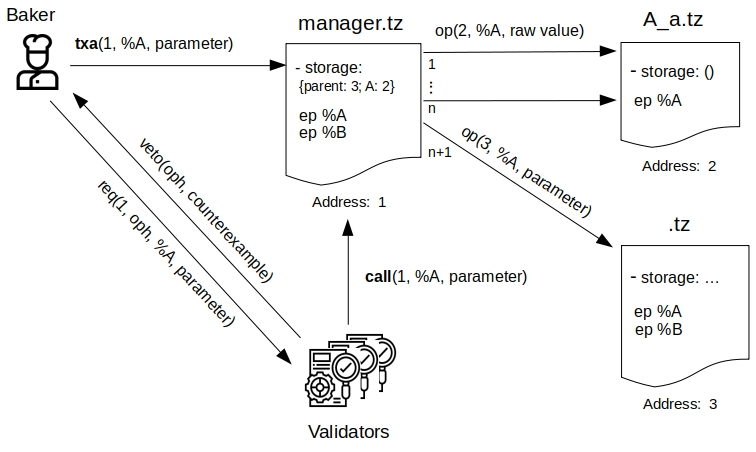
\includegraphics[width=0.9\textwidth]{figures/4-offline_tezos/interaction_modular.jpg}
	\caption{Interaction with a modular contract}
	\label{fig:interaction_modular}
\end{figure}

\subsubsection{Evaluation of the modular approach}
This approach fixes the two central problems of the monolithic approach: by mirroring the interface of the parent contract, the parameters passed to the manager contract can be forwarded directly to the parent contract, regardless of whether the default or an explicit entrypoint was called. As sum type parameters are stripped to the raw values inside the code block (ref. \lstref{lst:mono}), they can be passed to the assertion contract without further ado. Furthermore, the parent contract does not need to be modified, which leads to a much simpler compilation process and allows to extend already originated contracts with assertions. Due to its modularity, adaptions to either contract do not entail the recompilation and origination of all components. The manager is the only component with tight coupling, thus adaptions regarding the manager do not affect any other component. Adaptions to single assertions or the parent affect themselves plus the manager. In order to optimize this and break the tight coupling, one could be inclined to add a setter entrypoint to the manager (as a sort of dependency injection). This, however, would break the mirroring of the parent contract and is thus not possible without annulling one of the key strengths of the design.\\
The approach essentially has to weaknesses: on the one hand, the assertion and the parent cannot be called separately, as they are linked together by the manager. As a result, both the baker and validators execute the assertion, as well as the parent contract, which increases the cost of the contract execution. On the other hand, it exposes a security vulnerability, given that assertions can be bypassed by calling the parent contract directly with unevaluated parameters. This iteration of the design 
does not demand to close this vulnerability, hence possible solutions are not discussed in this thesis.

\section{Backend of the pipeline}
The Tezos backend of the pipeline comprises of the three stages semantic check, type check and compilation. During the semantic check, the common AST is cast to a Tezos-specific AST type. If the assertion contains any data types or operations not supported in Michelson, the assertion contract is rejected. Since the subsequent stages are less straight forward, they are explained in more detail in the following.
\begin{figure}[h]
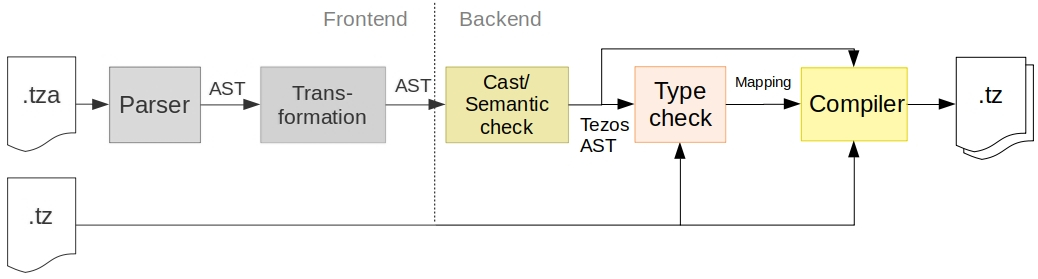
\includegraphics[width=\linewidth]{figures/4-offline_tezos/pipeline_backend}
\caption{The stages of Tezos-specific backend of the compilation pipeline}
\label{fig:pipeline_backend}
\end{figure}

\subsection{Type check}
The task of the type checker is to map the assertions from the given file to the respective entrypoints of the parent contract. To this end, the parameter types have to be compared and matched against each other in order to find a correct assignment. The type checker either reads the code of the parent contract from a given file or retrieves the code from a given address on the blockchain. It must be ensured that the created mapping is injective and unambiguous, i.e., each assertion matches exactly one entrypoint and no entrypoint is covered by more than one assertion.\\
As explained in \secref{sec:tezos}, entrypoints can be selected by calling the default entrypoint and wrapping the parameter into the respective union constructors. Alternatively, they can be called explicitly using their tag and passing the parameter as raw value. The same applies for the assertions - by omitting the tag, the parameter type must be declared in respect to the default entrypoint type. If the assertion states an explicit tag, it may declare the raw parameter type. The tags do not necessarily have to be identical with the tags of the parent contract; in some cases, they may be chosen differently for documentation or for readability purposes. However, the tags can and should be used to resolve ambiguity in the mapping between assertions and entrypoints, that is if several entrypoints share the same input type. Ambiguity can also be caused by the fact that entrypoints can be sub-entrypoints of others, thus assertions overlap if a separate assertion is declared for both super- and sub-entrypoint. This is resolved by detecting overlapping assertions during the type check and rejecting assertion contracts where appropriate. \\
As an exemplification, consider a Michelson contract with five entrypoints (including the \texttt{\%default}):
\begin{lstlisting}[numbers=none, language=Michelson]
parameter (or (int %A) (or %BC (int %B) (int %C)))
\end{lstlisting}
The following assertion contract for the given PC contains some valid and some invalid assertions:
\begin{lstlisting}[language=Assertion]
(assertion %A (i : int) ...)             (* valid *)
(assertion %D (i : int) ...)             (* invalid *)
(assertion (right (left (i : int)) ...)  (* valid *)
(assertion %BC (x : (or int int)) ...)   (* invalid *)
\end{lstlisting}
Due to its tag, the fist assertion can be assigned unambiguously to entrypoint A, whereas for the second it is not apparent whether it should be assigned to entrypoint B or C. Since the tag is omitted in the third assertion, the parameter type is given in respect to the default entrypoint and is assigned to B. The last assertion is invalid because it is overlapping with the previous assertion, which was already assigned to entrypoint B.

\subsection{Compiler}
The transformed and type checked assertion AST needs to be retargeted to Michelson code according to the orchestration scheme. Since the modular approach is less complex to implement and avoids having to decompile the parent code, this section describes a compiler that assembles the assertion and contract code according to \figref{fig:modular_assembly}. The target language of the compiler of the pipeline can either be Michelson directly, or another high-level language which supports Michelson as a target. \secref{sec:tezos} lists some examples of such languages. The chosen language then serves as an intermediate representation (IR) of the assertion and manager code, which is ultimately compiled to Michelson by the compiler of the language. After specifying the steps of the compilation in a general way, the compilation approaches are described and discussed in more detail in \secref{sec:direct} and \ref{sec:IR}.

\subsubsection{Compilation of the assertion contracts}
Since the assertions are independent of each other and the manager code, each of them can be compiled in isolation to a separate Michelson program. The generated code of the assertion body and the parameter type can be plugged into a template that already contains the necessary boilerplate code for a contract.

\subsubsection{Compilation of the manager contract}
Given that the manager contract mirrors the parent contract and assuming that the proposal for the storage type from \lstref{lst:manager_modular} is adopted, the type declarations can be translated directly to the target language. Algorithm \ref{alg:compile_manager} shows the outline of a simplified algorithm that builds the code body recursively. For simplicity, entrypoints that take a sum type as parameter (e.g. \texttt{(or \%AB int int)} are not considered in the algorithm. However, in the actual compiler implementation they need to be taken care of. 
\begin{algorithm}
\caption{Simplified recursive algorithm for building the manager contract}\label{alg:compile_manager}
	\begin{algorithmic}[0]
	\State global storage = \{0: <parent>\} \Comment{Stores the mapping of ids to entrypoints}
	\State global i = 1 \Comment{Counter generating unique ids}
	\Function{compile}{parent parameter type}
	\If{ty = Or(l,r)}
	\State code\_left = compile(l)
	\State code\_right = compile(r)
	\State \Return code\_left + code\_right
	\Else
	\If{assertion exists for this entrypoint}
	\State code = generate\_loop(ty, i)
	\State storage.add(i++, entrypoint tag)
	\Else
	\State code = generate\_forward(ty)
	\EndIf
	\State \Return code
	\EndIf
	\EndFunction
	\end{algorithmic}
\end{algorithm}

The function \texttt{generate\_loop} generates code that does the following:
\begin{enumerate}
\item Retrieve the assertion contract and parent contract addresses from storage
\item Calculate $t$
\item Build a list of $t$ internal operations that call the assertion contract
\item Return the list of emitted operations and the unchanged storage
\end{enumerate}
By passing the next id $i$ to the function, the access to the storage can be hard-wired into the generated code. The address of the parent contract is assumed to always be stored with the id 0. \secref{sec:prob_threshold} stated a formula for calculating $t_total$ with the parameters $n$, the size of the search space, and the probability threshold $c$. While $n$ can be calculated from the ranges of the random generator(s), $c$ must be given as parameter to the compiler through the CLI. After $t_total$ has been computed, a divison by 32, i.e., the number of validators, returns the upper bound of the loop. \\
\texttt{generate\_forward} can be generated from a simple template with the id as the only variant and only consists of  an access to the storage and the emission of an internal operation.

\subsubsection{Output}
Besides the target code for the manager and assertion contracts, the compiler should return a piece of template code for the correct storage initialization of the manager. Since this code is passed to the origination operation, it must be in Michelson regardless of the compilation target language. The placeholders or accompanying info should be descriptive enough, s.t. the user can plug in the corresponding addresses after the origination of the parent and assertion contracts. For the example manager contract given in \secref{sec:modular}, the corresponding text output could be\\
\texttt{(Elt 0 <addr parent>; Elt 1 <addr A\_a>; Elt 2 <addr B\_a>)}.

\subsubsection{Direct compilation}\label{sec:direct}
With the direct approach, the compiler generates Michelson code and hence code for a stack machine. Based on the simplicity of stack machines and the assumption that it does not need to generate optimal code, the compiler is expected to be simple \cite{cs5641}\cite{ferr_compiler}\cite{wiki:stack_machine}. As already indicate in the general part, the resulting contracts contain repeating structures and patterns for each input, which can be exploited by using template code during compilation. After compilation, the Michelson programs can be sanity-checked by type checking them using the provided Tezos libraries.

\paragraph{Assertion contracts}
\lstref{lst:contract_templ} shows a possible template for an assertion contract - the placeholder \texttt{<?>} marks the locations where the individual code is inserted. Lines 3-5 prepare the stack, s.t. the parameter and storage are the two top elements. The lines below the placeholder for the body clean up the stack and leave it according to calling convention, i.e., the program returns an empty list of internal operations and the unit storage.
\lstinputlisting[label=lst:contract_templ, language=Michelson, caption=Template code for assertion contracts in Michelson, numbers=left]{listings/assertion_template.tz}

\paragraph{Manager contract}
The generation of the \texttt{parameter} and \texttt{storage} primitives is trivial --- the parameter type can be carried over directly from the parent contract, whereas the storage type is a constant (\texttt{(map int address)}). Based on the algorithm given previously, the code body is generated by nesting \texttt{IF\_LEFT} instructions recursively (cf. \lstref{lst:entrypoints}). The adapted algorithm is given in Algorithm \ref{alg:compile_manager_direct}.
\begin{algorithm}
\caption{Modification of algorithm \ref{alg:compile_manager} for direct compilation}\label{alg:compile_manager_direct}
	\begin{algorithmic}[0]
	\State ...
	\Function{compile}{parent parameter type}
	\If{ty = Or(l,r)} \Comment{Compile sum types to a branching}
	\State code\_left = "IF\_LEFT {" + compile(l) + "}"
	\State code\_right = "{" + compile(r) + "}"
	\State \Return code\_left + code\_right
	\EndIf
	\State ...
	\EndFunction
	\end{algorithmic}
\end{algorithm}

Owing to Michelson being a low-level language, the templates for the functions \texttt{generate\_loop} and \texttt{generate\_forward} go beyond the scope of this subsection. In order to provide an idea of how the generated code could look like, appendix \ref{apx:manager_michelson} contains two example contracts, one of which contains manager code for a non-empty and the other one for an empty assertion. The code was generated by the Liquidity compiler from two contracts written in Liquidity, as this provides a more compact and readable representation of the program logic. The corresponding source code can be found in \secref{sec:IR}.

\paragraph{Evaluation}
Compiling to Michelson directly is beneficial due of several reasons - the pipeline stays streamlined and outputs the final contracts ready for origination. It does not introduce dependencies to external tools and their support for new protocol versions of Tezos. Besides, the new instructions only have to be added to Tezos' protocol code, whereas using external tools and languages would need to be patched as well in order to support them. \\
When it comes to verifying the compiler and integration testing of the pipeline, however, the low-level output causes more complexity than a high-level output. Due to the extend and restricted readability of non-trivial Michelson programs, their correctness is not always apparent in an instant. Tests can, on the one hand, compare the output with verified target contracts for a range of inputs, which requires a lot of Michelson code written by hand for each input. They, in turn, can also be prone to errors. On the other hand, the generated contracts can be tested as a black box using the test frameworks provided by Tezos, which use sandboxed networks to interact with contracts-under-test.

\subsubsection{Compiling to an IR}\label{sec:IR}
Instead of generating Michelson code directly, the compiler could also generate code in one of the high-level languages that provide a compiler with Michelson as a target. The output of the pipeline is then passed to this compiler in order to retrieve the final contracts. If the toolchain of the intermediate language doesn't provide a programmatic interface, the pipeline thus has to be extended with a separate step of procedure, as shown in \figref{fig:pipeline_liq}. This section demonstrates the implementation of this approach on the basis of Liquidity, hence the corresponding file extension \texttt{.liq}.
\begin{figure}[h]
\centering
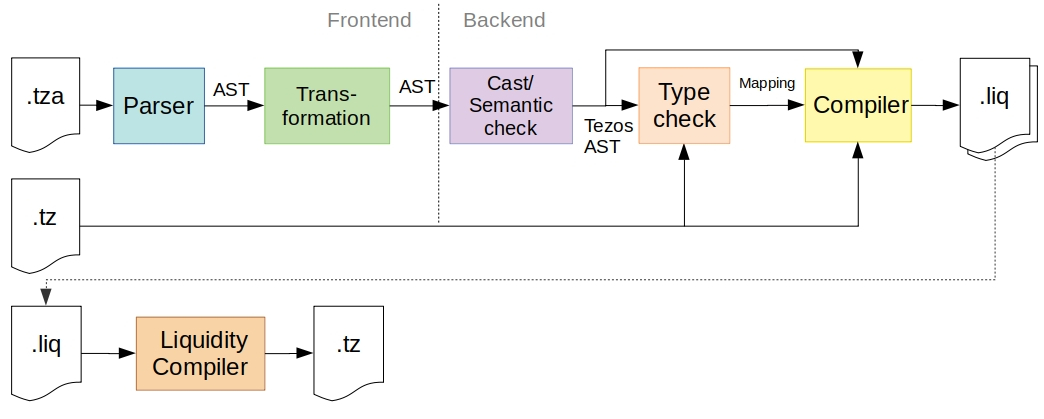
\includegraphics[width=\linewidth]{figures/4-offline_tezos/pipeline_liq}
\caption{Pipeline with IR compilation and an external toolchain}
\label{fig:pipeline_liq}
\end{figure}

\paragraph{Assertion contracts}
\lstinputlisting[label=lst:contract_templ_liq, language=Michelson, caption=Template code for assertion contracts in Liquidity, numbers=left]{listings/assertion_template.liq}

\paragraph{Manager contract}
\lstinputlisting[label=lst:manager_templ_liq, language=Michelson, caption=Manager code in Liquidity for an entrypoint with a non-empty assertion, numbers=left]{listings/manager_loop.liq}

\lstinputlisting[label=lst:manager_templ_liq, language=Michelson, caption=Manager code in Liquidity for an entrypoint with an empty assertion, numbers=left]{listings/manager_forward.liq}

\paragraph{Evaluation}
+ optimization (Liq compiler)
+ testing: easier to verify correctness, as it reads like an ocaml program
	+ compiler of hl language already tested -> only check if IR is correct
+ variable support -> variables in assertion easier to implement?


\section{Misc}
\todo{Aspects/questions I don't know yet if or where to put it}
\begin{itemize}
\item Tezos specific costs analysis of chosen orchestration strategy -> PROBLEM: high n might reach operation gas limit?
\item Representation of counterexamples; how to verify them?
\item Basic approach for proofs?
\end{itemize} 
    \chapter{Conclusion and outlook}\label{chap:conclusion}
In order to make use of off-chain computations in smart contracts, this thesis proposed an approach that engages the validators of the blockchain network in a distributed effort to check assertions over input parameters. It identified a set of properties, that can be checked in such a scheme, in form of logical formulas and demonstrated some use-cases and semantic differences among them. Based on this, a simple syntax was introduced to express assertions stating these formulas for a one or more entrypoints of a contract, followed by a formalization of their transformation that negates the formula and builds smart random generators. After analysing the accuracy of the approach and stating a formula to compute the minimum amount of random checks to reach a certain confidence level, the thesis explored several orchestration strategies of contract and assertion code, and, for a chosen strategy, discusses the necessary implementations within the off-chain infrastructure. In conclusion, it analysed the cost incurred by checking assertions as proposed and compared the results to a non-distributed approach. Based on these results, thesis discusses alternatives or possible modifications to solve some of the issues at hand. \\


- high costs due to several reasons: random checking values require more test runs than size of iteration space. going below n checks does not provide a high certainty over validity. This approach is thus not suitable for safety or security critical applications. 
- more effort in compilation returns a better cost-performance ratio if the manager contract and assertions are merged. Still, more base costs
- depends on the protocol design, whether this approach is worth pursuing -> if the cost for validation can be eliminated by using rewards, it might be realisable.
- quantifiers: other semantics for certain combinations/existentials --> proofs; here not considered, but would be interesting for future work on this topic

\subsection{Outlook}

\draft{}
\begin{itemize}
\item Summarize what has been implemented so far
\item Next steps
	\begin{itemize}
	\item extending VM \& Michelson
	\item compiler
	\item list open questions
	\item Protocol-design
		\begin{itemize}
		\item Do endorsers validate or extra validators?
		\item How to differentiate between SC w/ and w/o assertions?
		\item How to implement the waiting?
		\item Which transactions/messages can be reused or need to be introduced
		\item Representing counterexamples and verifying them
		\item Penalty for incorrect counterexamples
		\end{itemize}
	\end{itemize}
\item Estimation of cost reduction (or increase?)
\item Alternatives (e.g. TrueBit)
\end{itemize}

	\newpage
	\addcontentsline{toc}{chapter}{Appendix}
%	\fancyhead[R]{Appendix} %Kopfzeile links
	\appendix
\chapter{Assertion Grammar in EBNF}\label{apx:grammar}
The following two versions of the grammar implement the prefix and infix notations for the assertion syntax. 
\todo{Rename mutez}

\section{Prefix notation}
\lstinputlisting[basicstyle=\linespread{1.0}\fontfamily{lmr}\selectfont\small,
				 backgroundcolor=\color{cverbbg},
				 linewidth=14cm,
				 xleftmargin=0.5cm,
				 frame=lr,
				 framesep=8pt,
				 framerule=0pt,
				 captionpos=b,
				 numbers=none,
				 language=,
				 caption=Assertion grammar with prefix notation]{../grammar/assertion_grammar_prefix.txt}

\section{Infix notation}
\lstinputlisting[basicstyle=\linespread{1.0}\fontfamily{lmr}\selectfont\small,
				 backgroundcolor=\color{cverbbg},
				 linewidth=14cm,
				 xleftmargin=0.5cm,
				 frame=lr,
				 framesep=8pt,
				 framerule=0pt,
				 captionpos=b,
				 numbers=none,
				 language=,
				 caption=Assertion grammar with infix notation]{../grammar/assertion_grammar_infix.txt}

\chapter{List accessing in Michelson}\label{apx:nth}

\lstinputlisting[basicstyle=\linespread{1.0}\fontfamily{lmr}\selectfont\small,
				 backgroundcolor=\color{cverbbg},
				 linewidth=14cm,
				 xleftmargin=0.5cm,
				 frame=lr,
				 framesep=8pt,
				 framerule=0pt,
				 captionpos=b,
				 numbers=none,
				 language=,
				 label=lst:nth_liq,
				 caption=Possible implementation of \texttt{nth} in Liquidity]{listings/nth.liq}
				 
\lstinputlisting[basicstyle=\linespread{1.0}\fontfamily{lmr}\selectfont\small,
				 backgroundcolor=\color{cverbbg},
				 linewidth=14cm,
				 xleftmargin=0.5cm,
				 frame=lr,
				 framesep=8pt,
				 framerule=0pt,
				 captionpos=b,
				 numbers=none,
				 language=,
				 label=lst:nth_tz,
				 caption=\lstref{lst:nth_liq} compiled to Michelson]{listings/nth.tz}
    
    % bibliography is not in the table of contents per default, add it manually
    % enable the \renewcommand for german header
    % \renewcommand{\bibname}{Literaturverzeichnis}
    \addcontentsline{toc}{chapter}{Bibliography}

    \bibliographystyle{plain}
    \bibliography{bib/1-introduction,bib/2-use_case_analysis,bib/3-offline,bib/4-offline_tezos}
    \newpage
    \thispagestyle{empty}
    \mbox{}


\end{document}